\documentclass[20pt]{beamer}
\usepackage{fontspec}
\usepackage{amsfonts}
\usepackage{tangocolors}
\usepackage{listings}
\usepackage{hyperref}
\usepackage{multicol}
\usepackage{fontawesome}

\usepackage{tikz}
\usetikzlibrary{shapes}
\usetikzlibrary{backgrounds}
\usetikzlibrary{tikzmark}
\usetikzlibrary{decorations.pathmorphing}
\usetikzlibrary{positioning}
\usetikzlibrary{matrix}
\usetikzlibrary{math}

% thanks http://en.wikibooks.org/wiki/LaTeX/Packages/Listings
\newcommand\normallistingstyle{\lstset{ %
  language=Python,                % the language of the code
  basicstyle=\footnotesize,
                                   % the size of the fonts that are used for the code
  %numbers=left,                   % where to put the line-numbers
  %numberstyle=\tiny\color{gray},  % the style that is used for the line-numbers
  %stepnumber=1,                   % the step between two line-numbers. If it's 1, each line 
                                  % will be numbered
  %numbersep=5pt,                  % how far the line-numbers are from the code
  backgroundcolor=\color{white},      % choose the background color. You must add \usepackage{color}
  showspaces=false,               % show spaces adding particular underscores
  showstringspaces=false,         % underline spaces within strings
  showtabs=false,                 % show tabs within strings adding particular underscores
  %frame=single,                   % adds a frame around the code
  rulecolor=\color{black},        % if not set, the frame-color may be changed on line-breaks within not-black text
  tabsize=2,                      % sets default tabsize to 2 spaces
  %captionpos=b,                   % sets the caption-position to bottom
  breaklines=true,                % sets automatic line breaking
  breakatwhitespace=false,        % sets if automatic breaks should only happen at whitespace
  title=\ ,
  emph={[2]__import__,range,input,raw_input,NameError,dir,dict},
  keywordstyle=\color{ta3chocolate},          % keyword style
  commentstyle=\color{ta3orange},       % comment style
  stringstyle=\color{ta3orange},         % string literal style
  emphstyle={[2]\color{ta2orange}},
  escapeinside=\$\$,            % if you want to add LaTeX within your code
  morekeywords={*,...}               % if you want to add more keywords to the set
  aboveskip=0pt,
  belowskip=0pt,
}}
\newcommand\biglistingstyle{\lstset{ %
    basicstyle=\small,
}}
\newcommand\altlistingstyle{\lstset{ %
    backgroundcolor=\color{black},
    basicstyle=\small\color{white},
    keywordstyle=\color{tachocolate},
    commentstyle=\color{tachameleon},
    stringstyle=\color{tachameleon},
    emphstyle={[2]\color{tabutter}},
    emphstyle={[3]\color{taorange}},
}}
\normallistingstyle
\newcommand\topshade{
    \begin{tikzpicture}[remember picture,overlay]
    \fill[black] (current page.west) rectangle +(100cm, -100cm);
    \end{tikzpicture}
    \vspace{-50pt}
    \biglistingstyle
}
\newcommand\halfshadenopause{
    \altlistingstyle\bigskip\bigskip\bigskip
}
\newcommand\halfshade{
    \pause\halfshadenopause
}
\newcommand\bottomshade{
    \normallistingstyle
}
\newcommand\sk{\par\bigskip\bigskip\par}
\newcommand\wh[1]{\only<#1>{\color{white}}}
\newcommand\tx[2]{\alt<#1>{\textcolor{ta3gray}}{\textcolor{ta3gray}}{\uncover<#1->{#2}}}
\newcommand\rd[2]{\alt<#1>{\textcolor{ta2plum}}{\textcolor{ta3gray}}{#2}}
\renewcommand\emph[1]{\textcolor{ta2plum}{#1}}

\newcommand\xxhuge{\fontsize{150}{160}\selectfont}
\newcommand\xhuge{\fontsize{120}{130}\selectfont}
\newcommand\xtiny{\fontsize{6}{7}\selectfont}

\newcommand\xcoord[1]{\paperwidth*(-(1/2)+#1/100)}

\newcommand\nodey[1]{\begin{tikzpicture}[baseline=(X.base)] \node[white,fill=black,draw=white] (X) {#1}; \end{tikzpicture}}
\newcommand\noden[1]{\begin{tikzpicture}[baseline=(X.base)] \node[black,fill=white,draw=black] (X) {#1}; \end{tikzpicture}}

\newcommand\attributionnode[1]{
    \node[above right,fill=black,fill opacity=0.2,text opacity=1,inner sep=2pt]
        at(current page.south west)
    {\textcolor{white}{\xtiny #1}};
}

\begin{document}
\fontspec[Numbers={Lining, Monospaced}]{TeX Gyre Pagella}
\color{ta3gray}

\begin{center}
\title{eval()}
\author{Petr Viktorin}
\date{\today}

\frame{\color{ta3gray}
    \sk
    \textcolor{ta2gray}{Jak postavit slovník \\ z jedniček a nul}
    \sk\sk
    \textcolor{ta2gray}{Petr Viktorin}\\[-0.25cm]
    \textcolor{ta2gray}{\tiny encukou.cz}\\[-0.5cm]
    \textcolor{ta2gray}{\tiny encukou@gmail.com}
    \sk
    \textcolor{ta2gray}{\tiny Brněnské Pyvo, 2016-09-29}
}

\frame[plain]{
    \leftskip-0.4in
    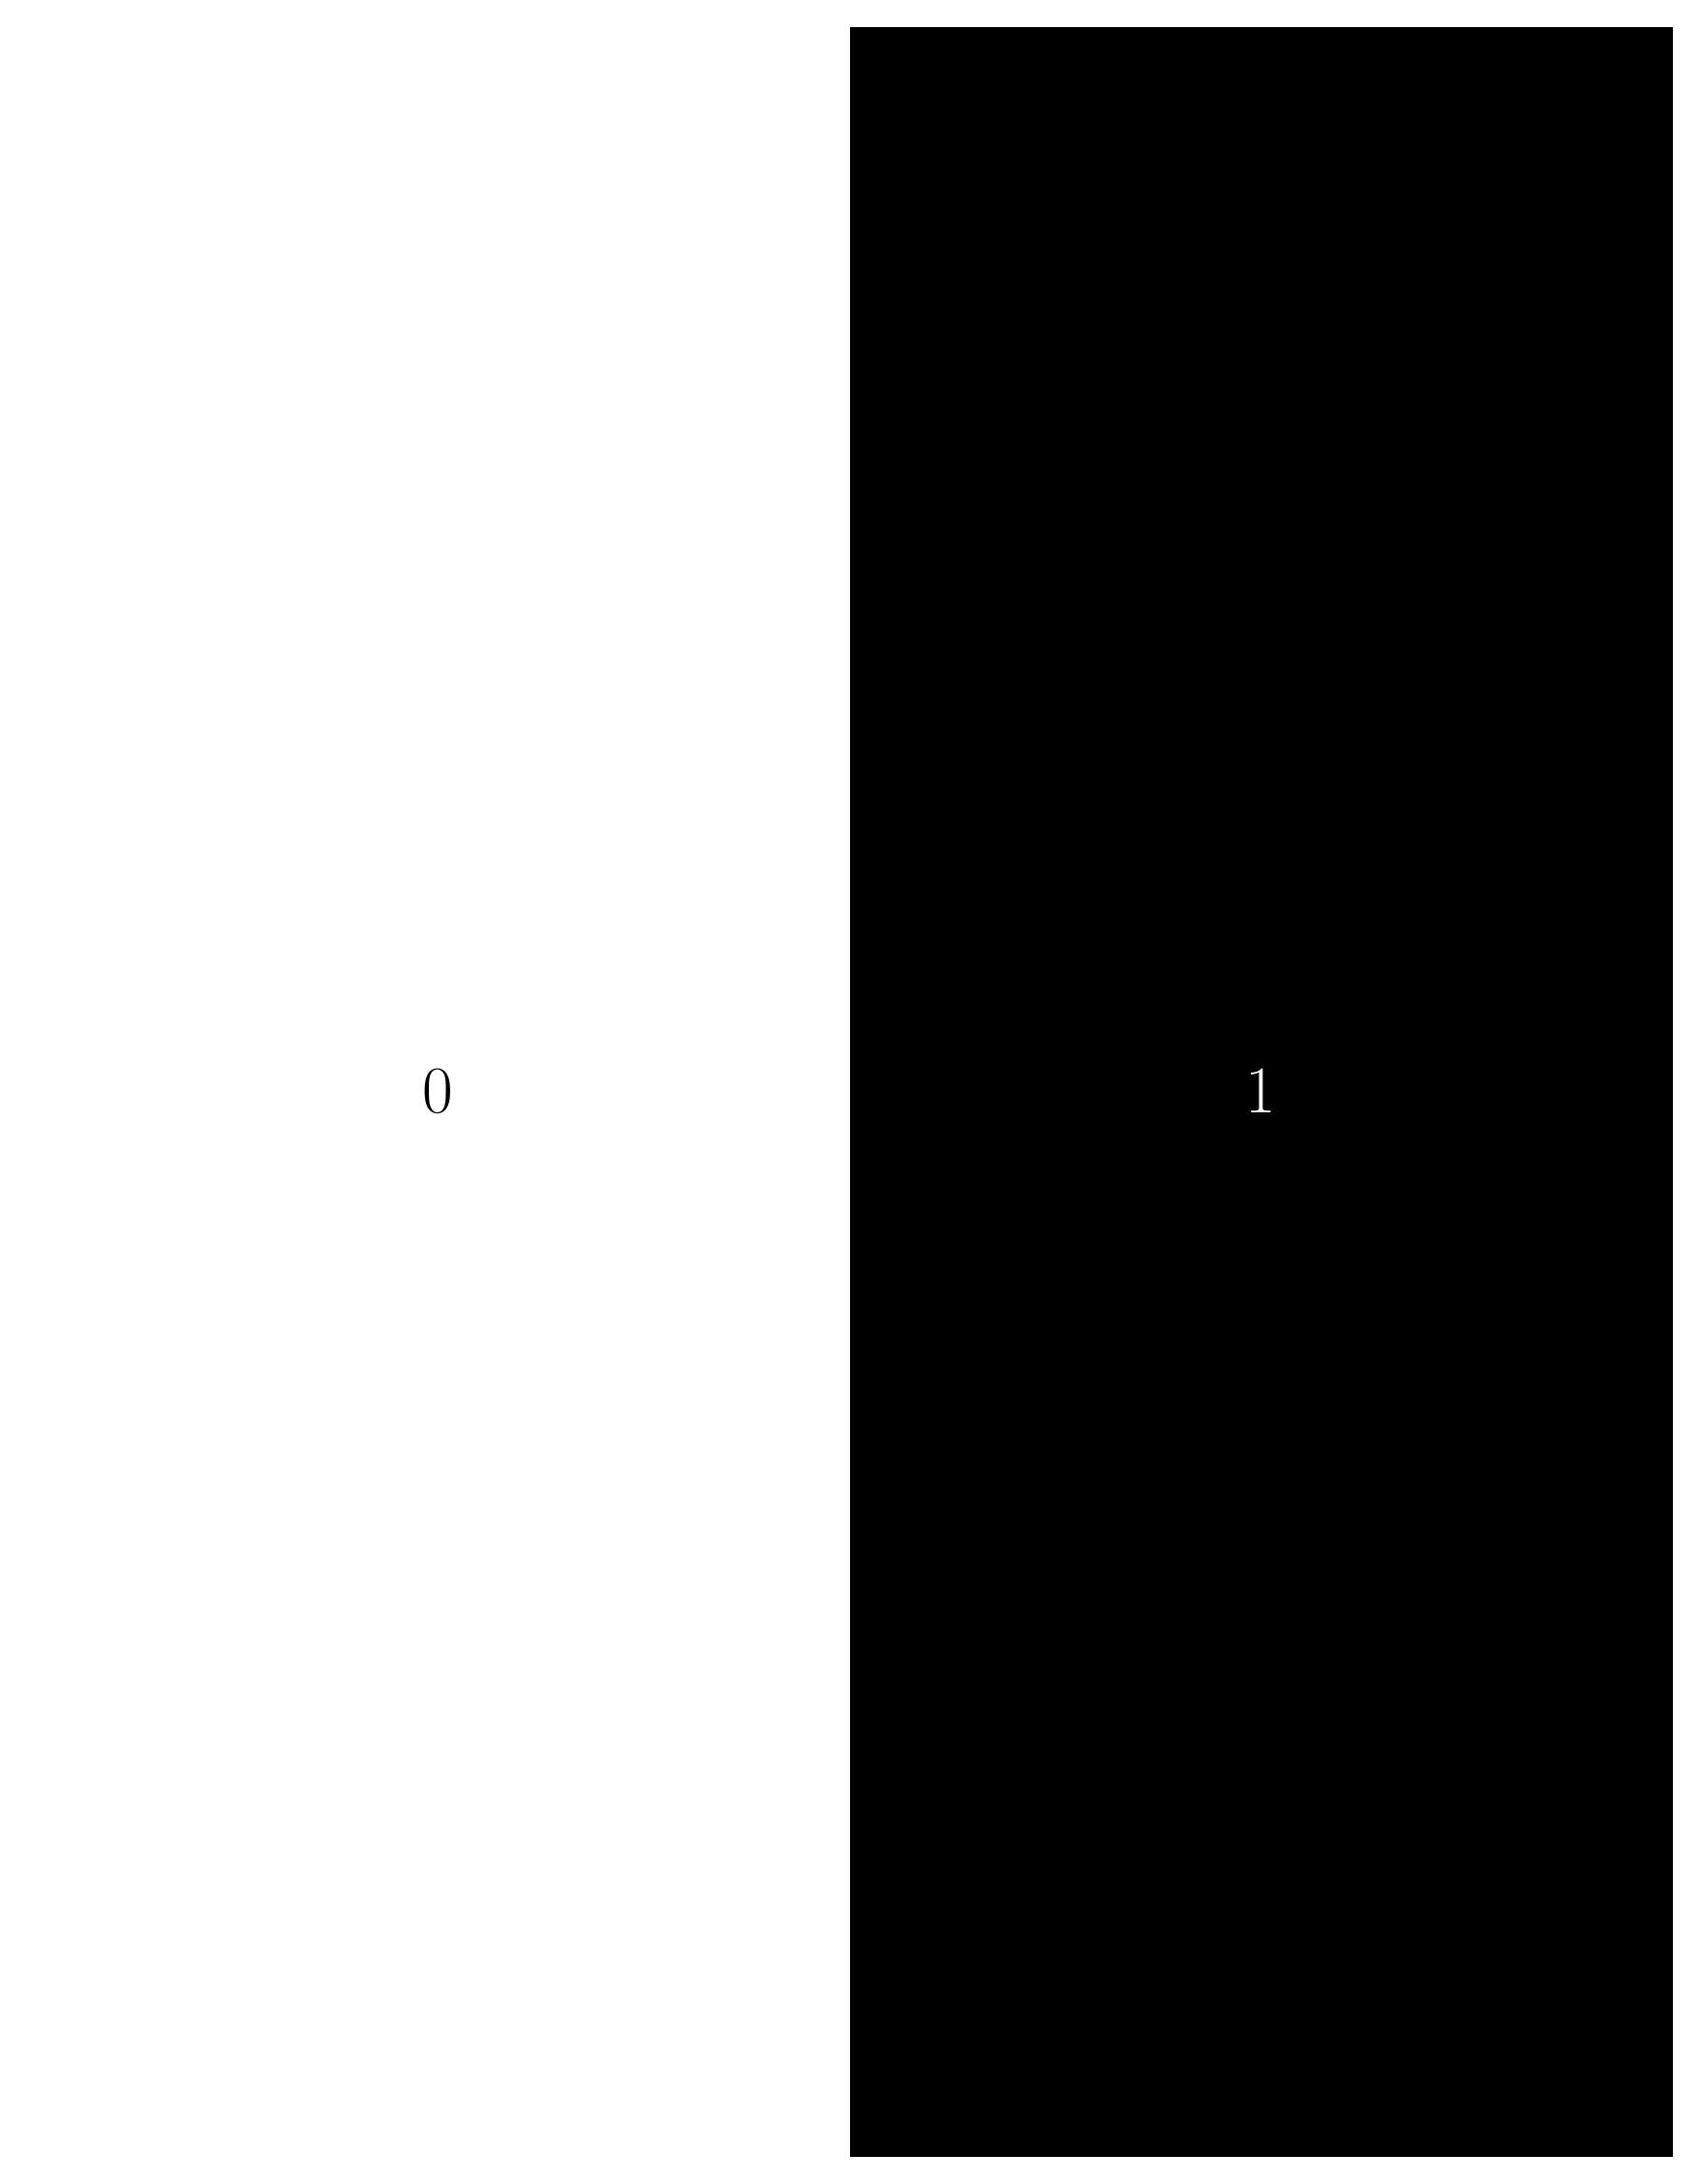
\begin{tikzpicture}
        \path[fill=white] (0,0) -- (-\paperwidth/2, 0) -- (-\paperwidth/2, \paperheight)
                    --  (0, \paperheight) -- cycle;
        \path[fill=black] (0,0) -- (\paperwidth/2, 0) -- (\paperwidth/2, \paperheight)
                    --  (0, \paperheight) -- cycle;
        \node[black] at (-\paperwidth/4, \paperheight/2) {\xxhuge 0};
        \node[white] at (\paperwidth/4, \paperheight/2) {\xxhuge 1};
    \end{tikzpicture}
}

\frame[plain]{
    \leftskip-0.4in
    \begin{tikzpicture}[remember picture]
        \path[fill=white] (0,0) -- (-\paperwidth/2, 0) -- (-\paperwidth/2, \paperheight)
                    --  (0, \paperheight) -- cycle;
        \path[fill=black] (0,0) -- (\paperwidth/2, 0) -- (\paperwidth/2, \paperheight)
                    --  (0, \paperheight) -- cycle;
        \node[black] at (-\paperwidth/4, \paperheight/3) {\xhuge 0V};
        \node[white] at (\paperwidth/4, \paperheight/3) {\xhuge 3V};
        \node at (0, \paperheight*3/4)
            {{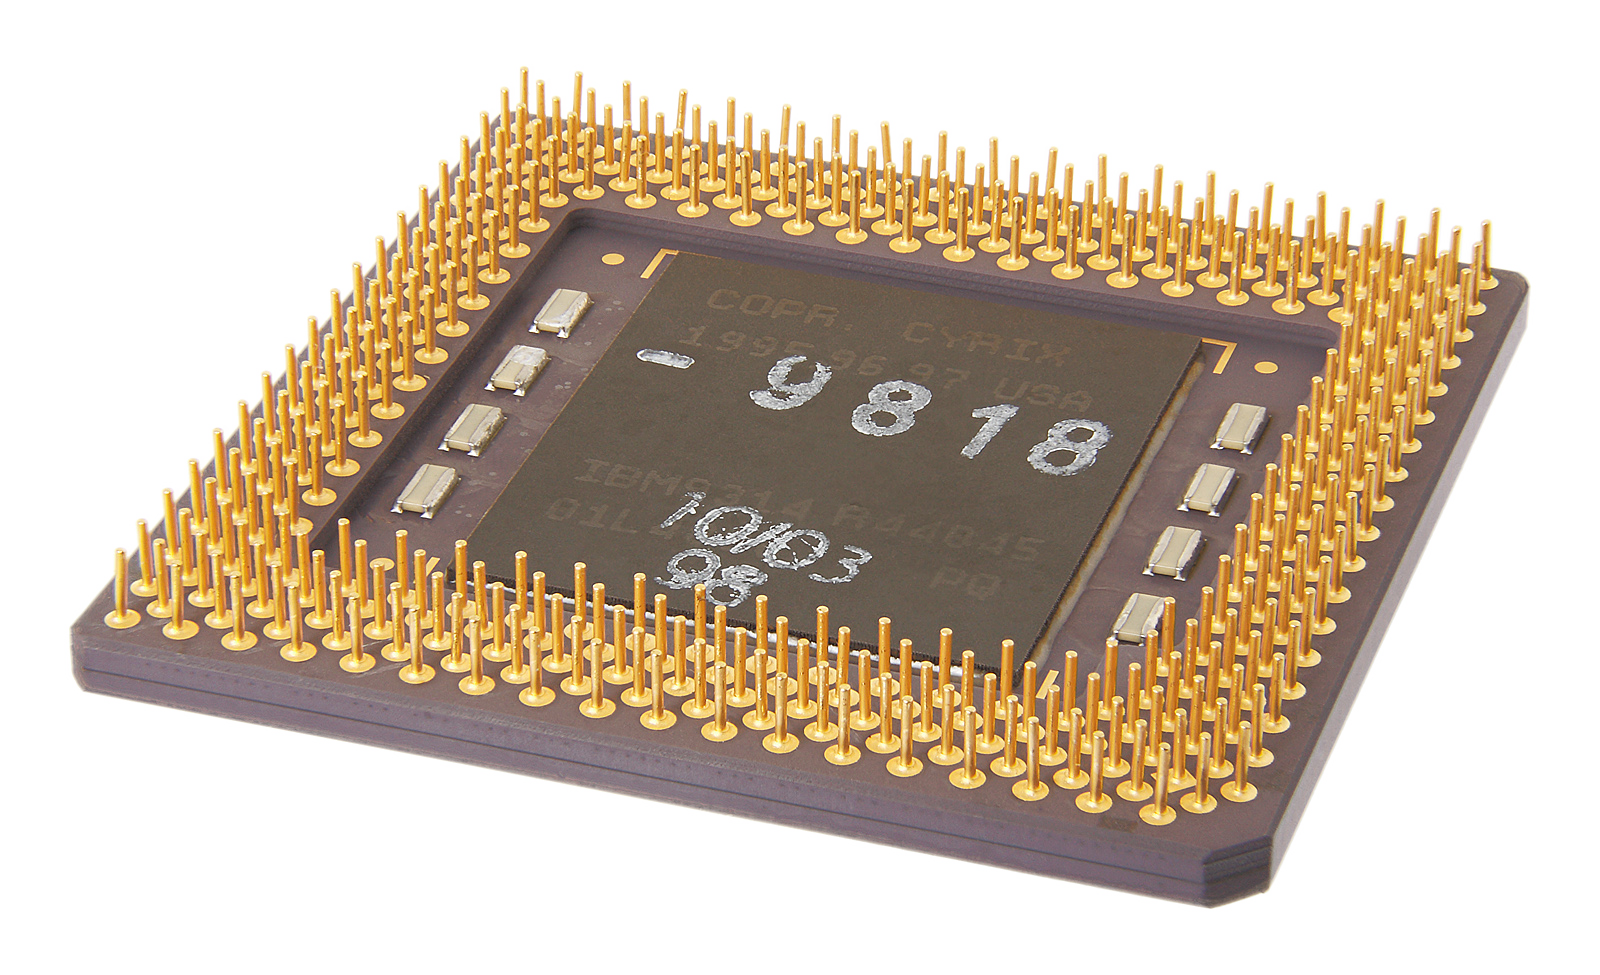
\includegraphics[width=5cm]{processor}}};
        % https://en.wikipedia.org/wiki/File:Cyrix_IBM_CPU_6x86MX_PR200_bottom.jpg
        % Eric Gaba, Wikimedia Commons user Sting
        % CC-BY-SA
        \attributionnode{Image © Eric Gaba, Wikimedia Commons user Sting, CC-BY-SA: \url{https://en.wikipedia.org/wiki/File:Cyrix_IBM_CPU_6x86MX_PR200_bottom.jpg}}
    \end{tikzpicture}
}

\frame[plain]{
    \leftskip-0.4in
    \begin{tikzpicture}
        \path[fill=white] (0,0) -- (-\paperwidth/2, 0) -- (-\paperwidth/2, \paperheight)
                    --  (0, \paperheight) -- cycle;
        \path[fill=black] (0,0) -- (\paperwidth/2, 0) -- (\paperwidth/2, \paperheight)
                    --  (0, \paperheight) -- cycle;
        \node[black] at (-\paperwidth/4, \paperheight/3) {\xhuge };
        \node[white] at (\paperwidth/4, \paperheight/3) {\xhuge \faCircle};
        \node at (0, \paperheight*3/4)
            {{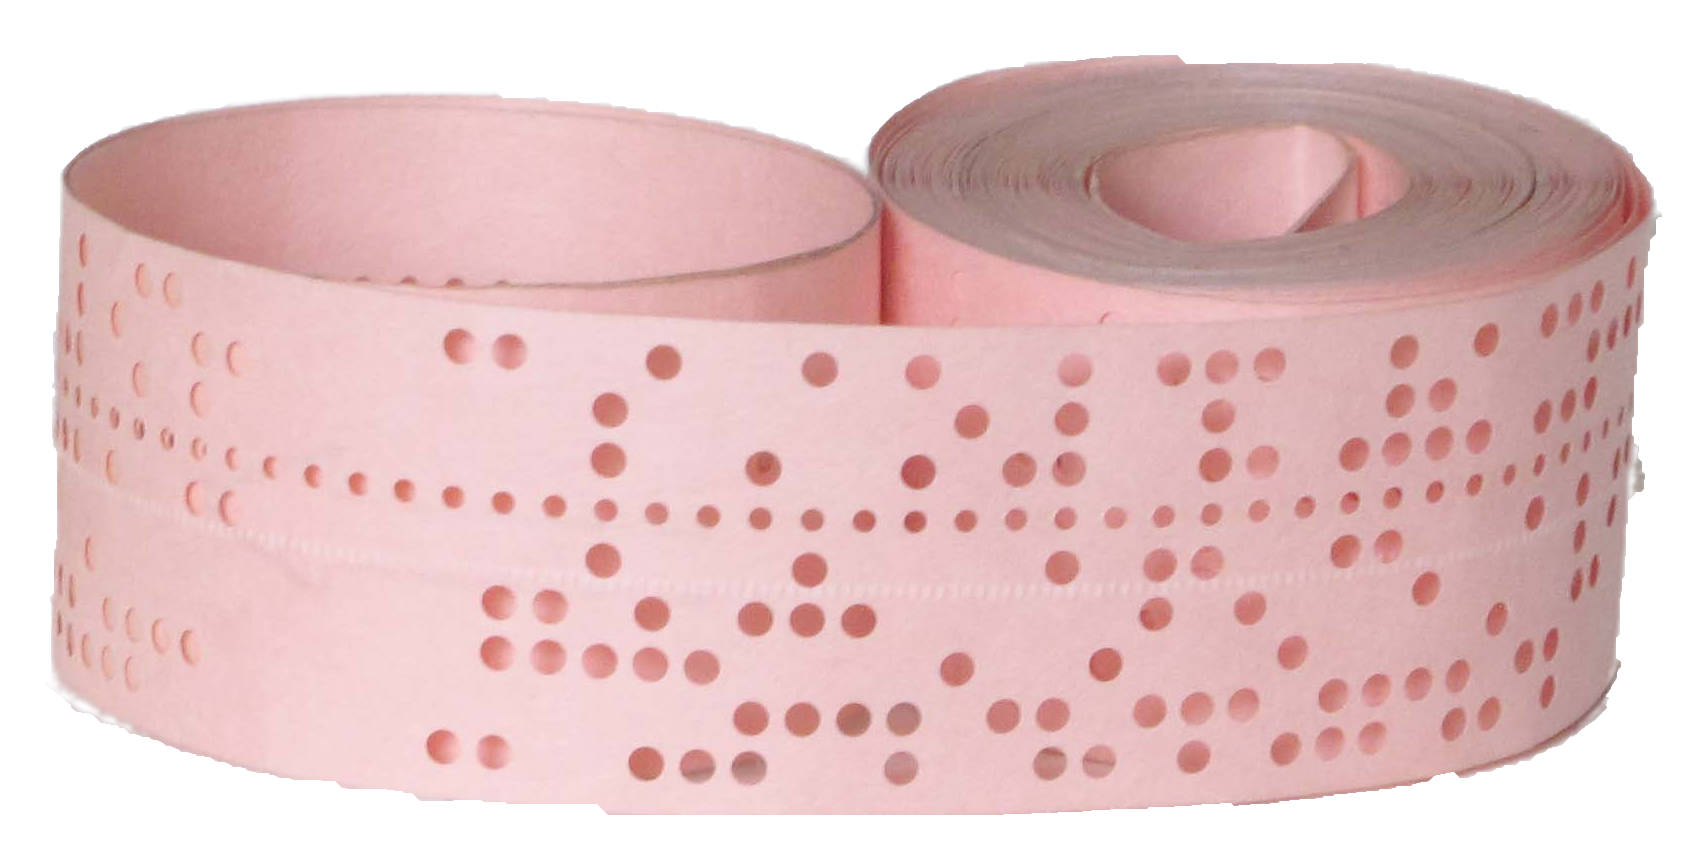
\includegraphics[width=8cm]{punched-tape}}};
        % https://en.wikipedia.org/wiki/File:PaperTapes-5and8Hole.jpg
        % Public Domain
    \end{tikzpicture}
}

\frame[plain]{
    \leftskip-0.4in
    \begin{tikzpicture}
        \path[fill=white] (0,0) -- (-\paperwidth/2, 0) -- (-\paperwidth/2, \paperheight)
                    --  (0, \paperheight) -- cycle;
        \path[fill=black] (0,0) -- (\paperwidth/2, 0) -- (\paperwidth/2, \paperheight)
                    --  (0, \paperheight) -- cycle;
        \node[black] at (-\paperwidth/4, \paperheight/3) {\xhuge S};
        \node[white] at (\paperwidth/4, \paperheight/3) {\xhuge J};
        \node at (0, \paperheight*3/4)
            {{
\includegraphics[width=4cm]{floppy-disk}}};
        % https://en.wikipedia.org/wiki/File:Floppy_disk_300_dpi.jpg
        % Public Domain
    \end{tikzpicture}
}

\frame[plain]{
    \leftskip-0.4in
    \begin{tikzpicture}
        \path[fill=white] (0,0) -- (-\paperwidth/2, 0) -- (-\paperwidth/2, \paperheight)
                    --  (0, \paperheight) -- cycle;
        \path[fill=black] (0,0) -- (\paperwidth/2, 0) -- (\paperwidth/2, \paperheight)
                    --  (0, \paperheight) -- cycle;
        \node[black] at (-\paperwidth/4, \paperheight/3) {\xhuge \faEye};
        \node[white] at (\paperwidth/4, \paperheight/3) {\xhuge \faEyeSlash};
        \node at (0, \paperheight*3/4)
            {{
\includegraphics[width=4cm]{dvd}}};
        % https://en.wikipedia.org/wiki/File:DVD-Video_bottom-side.jpg
        % Public Domain
    \end{tikzpicture}
}

\frame[plain]{
    \leftskip-0.4in
    \begin{tikzpicture}
        \path[fill=white] (0,0) -- (-\paperwidth/2, 0) -- (-\paperwidth/2, \paperheight)
                    --  (0, \paperheight) -- cycle;
        \path[fill=black] (0,0) -- (\paperwidth/2, 0) -- (\paperwidth/2, \paperheight)
                    --  (0, \paperheight) -- cycle;
        \node[black] at (-\paperwidth/4, \paperheight/3) {\xhuge \faRemove};
        \node[white] at (\paperwidth/4, \paperheight/3) {\xhuge \faCheck};
        \node at (0, \paperheight*5/7) {{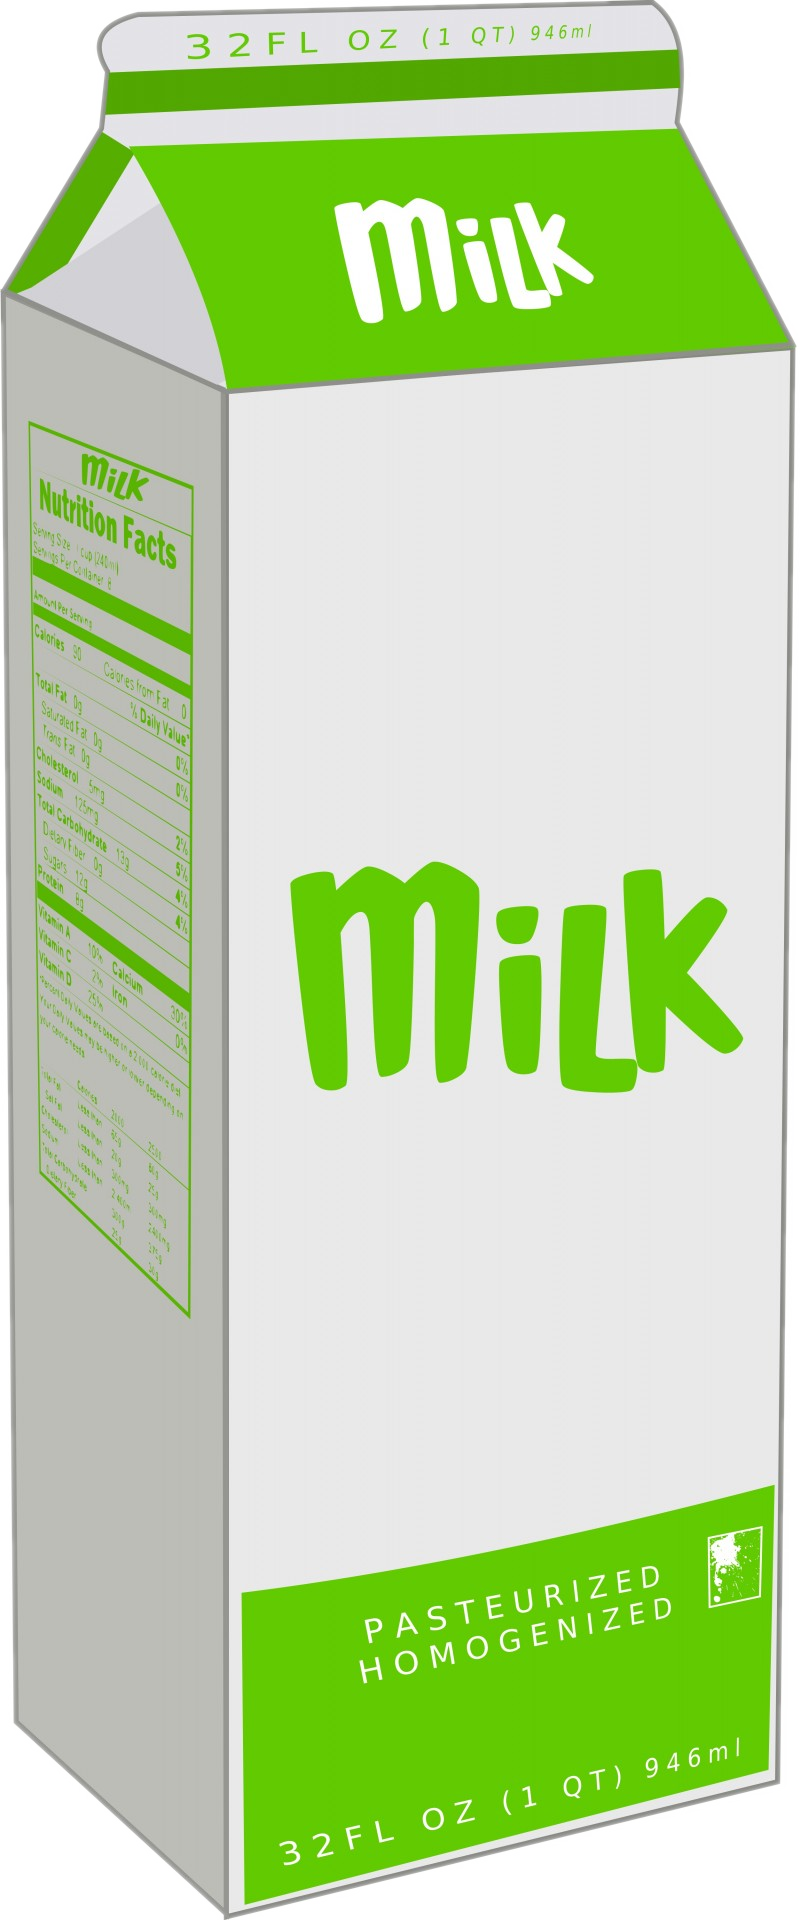
\includegraphics[width=2cm]{milk-carton}}};
        % http://www.publicdomainpictures.net/view-image.php?image=118101&picture=milk-carton
        % Public Domain
    \end{tikzpicture}
}

\frame[plain]{
    \leftskip-0.4in
    \begin{tikzpicture}
        \path[fill=white] (0,0) -- (-\paperwidth/2, 0) -- (-\paperwidth/2, \paperheight)
                    --  (0, \paperheight) -- cycle;
        \path[fill=black] (0,0) -- (\paperwidth/2, 0) -- (\paperwidth/2, \paperheight)
                    --  (0, \paperheight) -- cycle;
        \node[black] at (-\paperwidth/4, \paperheight/3) {\xhuge \faMars};
        \node[white] at (\paperwidth/4, \paperheight/3) {\xhuge \faVenus};
        \node at (0, \paperheight*5/7) {{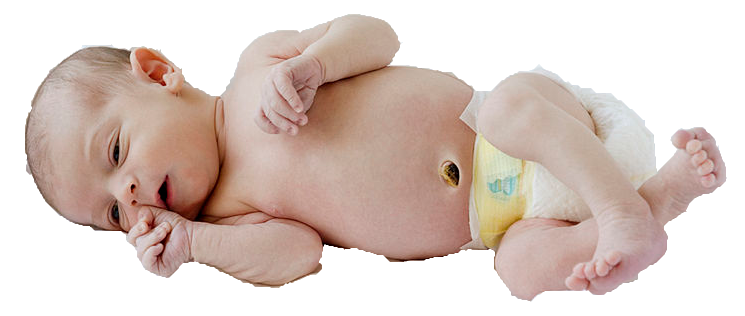
\includegraphics[width=6cm]{baby}}};
        % https://en.wikipedia.org/wiki/File:Human-Male-Newborn-Infant-Baby.jpg
        % Public Domain
    \end{tikzpicture}
}

\frame[plain]{
    \leftskip-0.4in
    \begin{tikzpicture}
        \path[fill=white] (0,0) -- (-\paperwidth/2, 0) -- (-\paperwidth/2, \paperheight)
                    --  (0, \paperheight) -- cycle;
        \path[fill=black] (0,0) -- (\paperwidth/2, 0) -- (\paperwidth/2, \paperheight)
                    --  (0, \paperheight) -- cycle;
        \node[black] at (-\paperwidth/4, \paperheight/3) {\xhuge \faLevelUp};
        \node[white] at (\paperwidth/4, \paperheight/3) {\xhuge \faLevelDown};
        \node at (0, \paperheight*5/7) {{
\includegraphics[width=3cm]{ladybug}}};
        % http://www.freestockphotos.biz/stockphoto/10710
        % Public Domain
    \end{tikzpicture}
}

\frame[plain]{
    \leftskip-0.4in
    \begin{tikzpicture}[remember picture]
        \path[fill=white] (0,0) -- (-\paperwidth/2, 0) -- (-\paperwidth/2, \paperheight)
                    --  (0, \paperheight) -- cycle;
        \path[fill=black] (0,0) -- (\paperwidth/2, 0) -- (\paperwidth/2, \paperheight)
                    --  (0, \paperheight) -- cycle;
        \node[black] at (-\paperwidth/4, \paperheight/3) {\xhuge \faHeart};
        \node[white] at (\paperwidth/4, \paperheight/3) {\xhuge \faFrownO};
        \node at (0, \paperheight*5/7) {{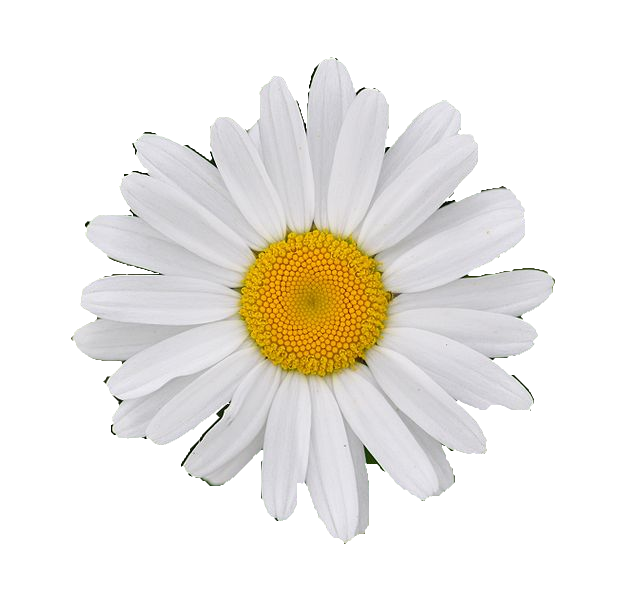
\includegraphics[width=4cm]{daisy}}};
        % https://commons.wikimedia.org/wiki/File:Leucanthemum_vulgare_qtl1.jpg
        % Wikimedia user Quartl
        % CC-BY-SA 3.0
        \attributionnode{Image © Wikimedia user Quartl, CC-BY-SA: \url{https://commons.wikimedia.org/wiki/File:Leucanthemum_vulgare_qtl1.jpg}}
    \end{tikzpicture}
}

\frame[plain]{
    \leftskip-0.4in
    \begin{tikzpicture}
        \path[fill=white] (0,0) -- (-\paperwidth/2, 0) -- (-\paperwidth/2, \paperheight)
                    --  (0, \paperheight) -- cycle;
        \path[fill=black] (0,0) -- (\paperwidth/2, 0) -- (\paperwidth/2, \paperheight)
                    --  (0, \paperheight) -- cycle;
        \node[black] at (-\paperwidth/4, \paperheight/3) {\xhuge \faSunO};
        \node[white] at (\paperwidth/4, \paperheight/3) {\xhuge \faCloud};
        \node at (0, \paperheight*5/7) {{
\includegraphics[width=4cm]{umbrella}}};
        % https://commons.wikimedia.org/wiki/File:Umbrella_opened.svg
        % Public Domain
    \end{tikzpicture}
}

\frame[plain]{
    \leftskip-0.4in
    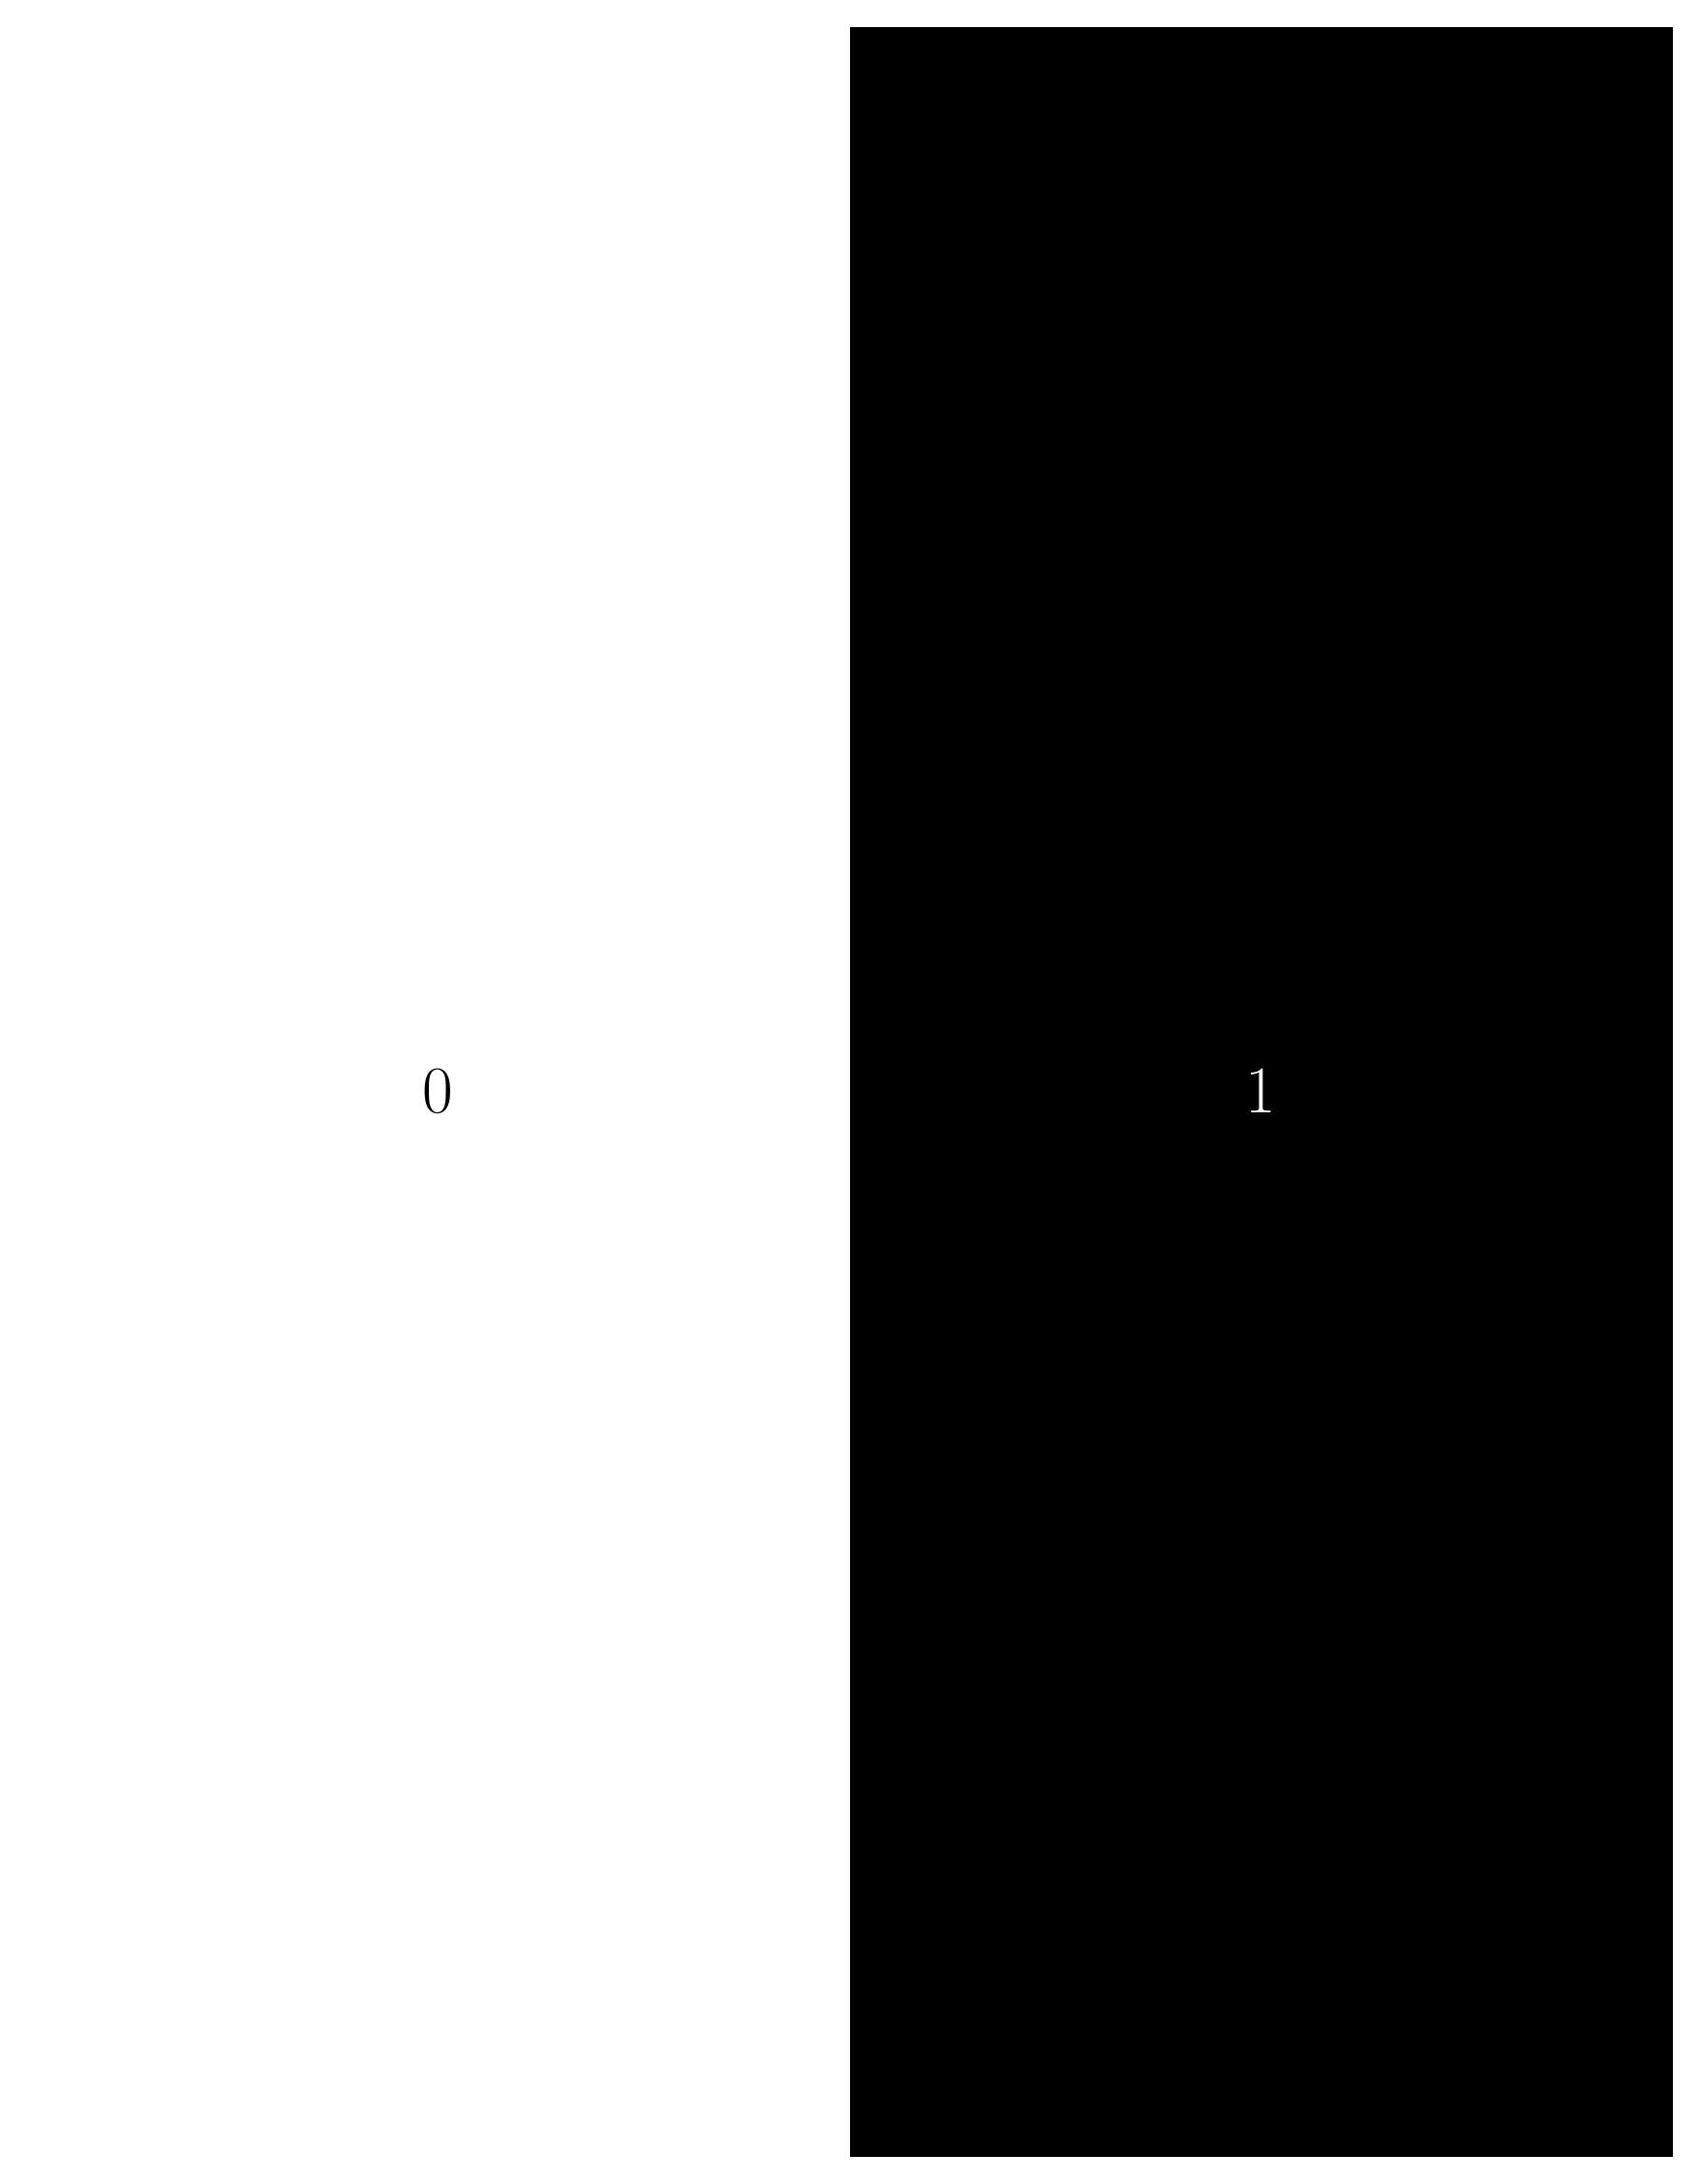
\begin{tikzpicture}
        \path[fill=white] (0,0) -- (-\paperwidth/2, 0) -- (-\paperwidth/2, \paperheight)
                    --  (0, \paperheight) -- cycle;
        \path[fill=black] (0,0) -- (\paperwidth/2, 0) -- (\paperwidth/2, \paperheight)
                    --  (0, \paperheight) -- cycle;
        \node[black] at (-\paperwidth/4, \paperheight/2) {\xxhuge 0};
        \node[white] at (\paperwidth/4, \paperheight/2) {\xxhuge 1};
    \end{tikzpicture}
}

\frame {

    {\huge Bude zítra pršet?}
    \pause

    \bigskip

    {\faCaretRight} Ano\\\pause
    {\faCaretRight} Ne\\\pause
    {\faCaretRight} Nevím\\\pause
    {\faCaretRight} S 40\% pravděpodobností\\\pause
    {\faCaretRight} Myslíš v Brně?\\\pause
    {\faCaretRight} Podle jakého modelu?
}

\frame[plain]{

    \bigskip

    {Umíš odpovědět „ano” nebo „ne” na otázku „Bude zítra pršet?”}

    \bigskip

    \pause
    \leftskip-0.4in
    
\begin{tikzpicture}[align=center]
        \path[fill=white] (0,0) -- (-\paperwidth/2, 0) -- (-\paperwidth/2, \paperheight)
                    --  (0, \paperheight) -- cycle;
        \path[fill=black] (0,0) -- (\paperwidth/2, 0) -- (\paperwidth/2, \paperheight)
                    --  (0, \paperheight) -- cycle;
        \node[black,below] at (-\paperwidth/4, \paperheight*7/8) {\faCheck \\ Bude zítra pršet?};
        \pause
        \node[white,below] at (\paperwidth/4, \paperheight*7/8) {\faRemove \\ Aha... \\ A je to tím \\ že to nevíš \\ přesně?};
    \end{tikzpicture}
}

\frame[plain]{

    \bigskip

    Kolik je mi let?

    \bigskip

    \leftskip-0.4in
    
\begin{tikzpicture}[align=center]
        \pause
        \path[fill=white] (0,0) rectangle (-\paperwidth/2, \paperheight);
        \path[fill=black] (0,0) rectangle (\paperwidth/2, \paperheight);
        \node[black,circle,fill=white,draw=black] at (0, \paperheight) {50};
        \pause
        \path[fill=gray] (0,0) rectangle (\paperwidth/2, \paperheight*0.9);
        \node[white] at (\paperwidth/4, \paperheight*0.8) {\faRemove};
        \pause
        \path[fill=white] (-\paperwidth/2,0) rectangle (-\paperwidth/4, \paperheight*0.9);
        \path[fill=black] (-\paperwidth/4,0) rectangle (0, \paperheight*0.9);
        \node[black,circle,fill=white,draw=black] at (-\paperwidth/4, \paperheight*0.9) {25};
        \pause
        \path[fill=gray] (-\paperwidth/2,0) rectangle (-\paperwidth/4, \paperheight*0.8);
        \node[white] at (-\paperwidth*3/8, \paperheight*0.7) {\faRemove};
        \pause
        \path[fill=white] ({\xcoord{25}},0) rectangle ({\xcoord{35}}, \paperheight*0.8);
        \path[fill=black] ({\xcoord{35}},0) rectangle ({\xcoord{50}}, \paperheight*0.8);
        \node[black,circle,fill=white,draw=black] at ({\xcoord{35}}, \paperheight*0.8) {35};
        \pause
        \path[fill=gray] ({\xcoord{35}},0) rectangle ({\xcoord{55}}, \paperheight*0.7);
        \node[white] at ({\xcoord{42.5}}, \paperheight*0.6) {\faRemove};
        \pause
        \path[fill=white] ({\xcoord{25}},0) rectangle ({\xcoord{30}}, \paperheight*0.65);
        \path[fill=black] ({\xcoord{30}},0) rectangle ({\xcoord{35}}, \paperheight*0.65);
        \node[black,circle,fill=white,draw=black] at ({\xcoord{30}}, \paperheight*0.65) {\tiny 30};
        \pause
        \path[fill=gray] ({\xcoord{30}},0) rectangle ({\xcoord{35}}, \paperheight*0.55);
        \pause
        \path[fill=white] ({\xcoord{25}},0) rectangle ({\xcoord{27}}, \paperheight*0.53);
        \path[fill=black] ({\xcoord{27}},0) rectangle ({\xcoord{30}}, \paperheight*0.53);
        \node[black,circle,fill=white,draw=black,inner sep=2pt] at ({\xcoord{27}}, \paperheight*0.53) {\tiny 27};
        \pause
        \path[fill=gray] ({\xcoord{20}},0) rectangle ({\xcoord{27}}, \paperheight*0.48);
        \pause
        \path[fill=white] ({\xcoord{27}},0) rectangle ({\xcoord{29}}, \paperheight*0.47);
        \path[fill=black] ({\xcoord{29}},0) rectangle ({\xcoord{30}}, \paperheight*0.47);
        \node[black,circle,fill=white,draw=black,inner sep=2pt] at ({\xcoord{29}}, \paperheight*0.47) {\tiny 29};
        \pause
        \path[fill=gray] ({\xcoord{29}},0) rectangle ({\xcoord{33}}, \paperheight*0.42);
        \pause
        \path[fill=white] ({\xcoord{27}},0) rectangle ({\xcoord{28}}, \paperheight*0.40);
        \path[fill=black] ({\xcoord{28}},0) rectangle ({\xcoord{29}}, \paperheight*0.40);
        \node[black,circle,fill=white,draw=black,inner sep=2pt] at ({\xcoord{28}}, \paperheight*0.40) {\tiny 28};
        \pause
        \path[fill=gray] ({\xcoord{20}},0) rectangle ({\xcoord{28}}, \paperheight*0.35);
    \end{tikzpicture}
}

\frame[plain]{

    \bigskip

    Myslím si číslo

    \bigskip

    \leftskip-0.4in
    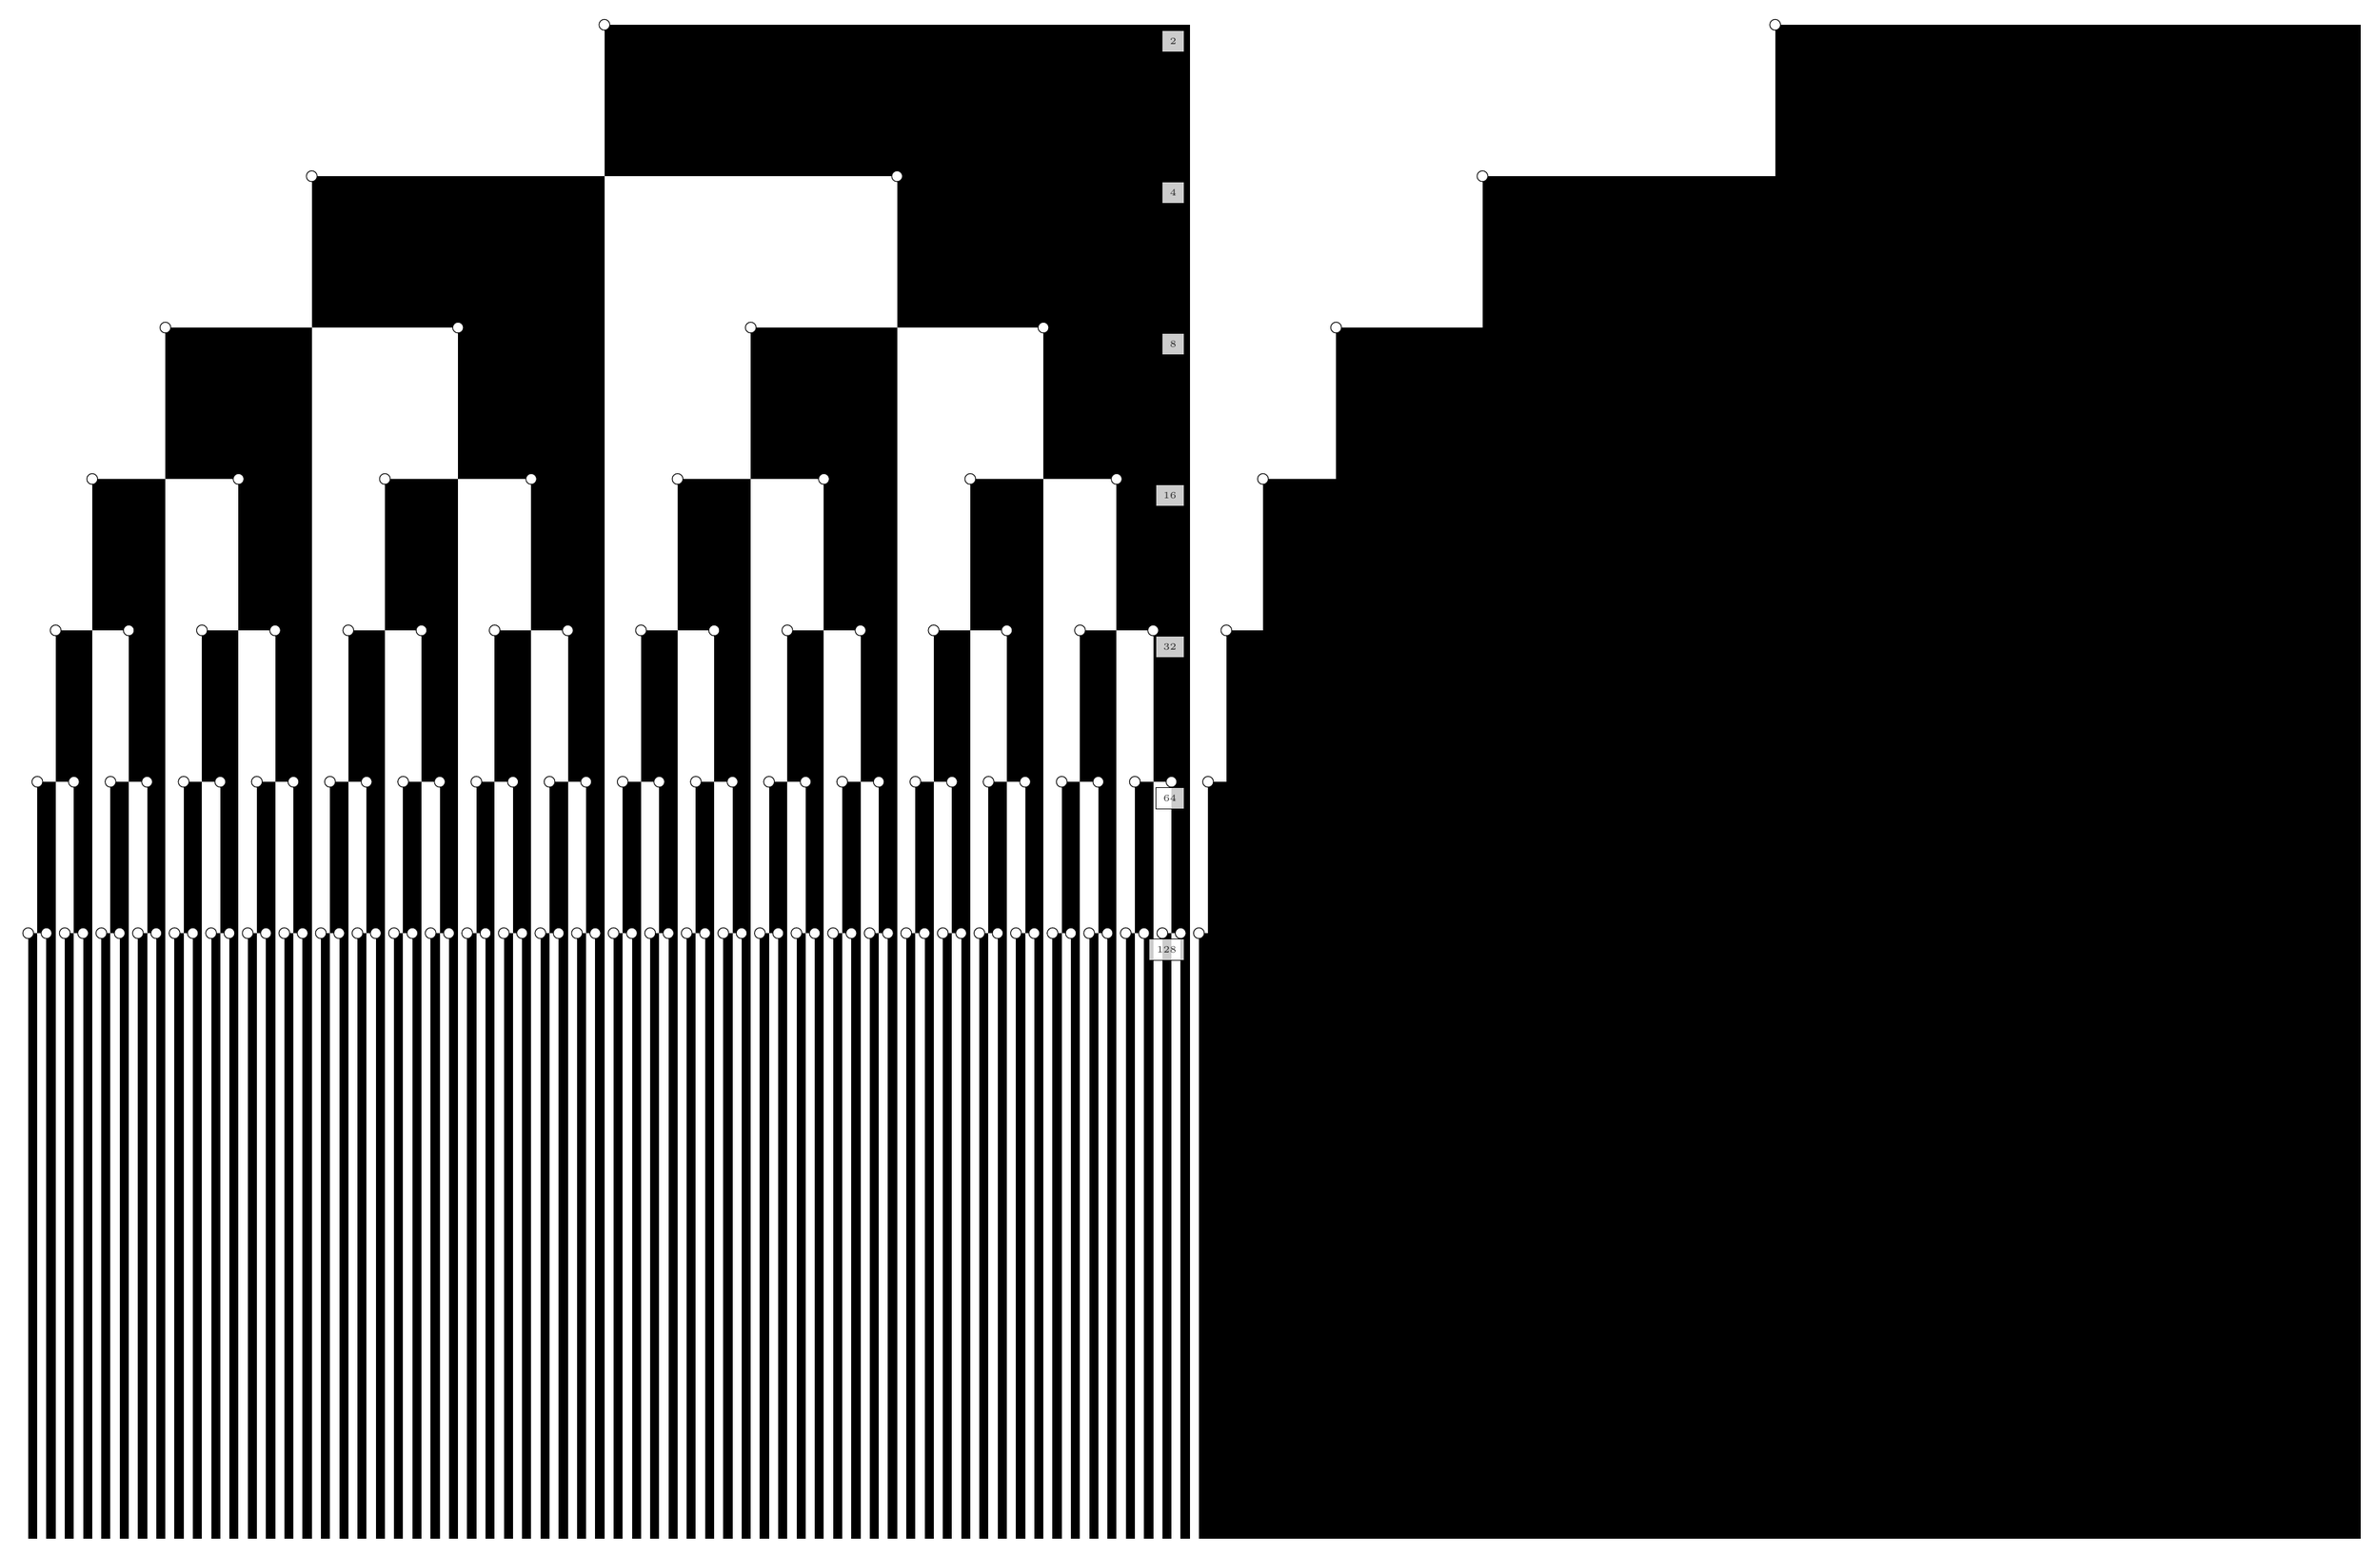
\begin{tikzpicture}[align=center]
        \foreach \m/\y in {1/1, 2/0.9, 4/0.8, 8/0.7,16/0.6,32/0.5,64/0.4} {
            \pause
            \foreach \x in {0,...,\m} {
                \path[fill=white] ({\paperwidth*(-1+(\x+0)/\m)},0) rectangle ({\paperwidth*(-1+(\x+.5)/\m)}, {\paperheight*\y});
                \path[fill=black] ({\paperwidth*(-1+(\x+.5)/\m)},0) rectangle ({\paperwidth*(-1+(\x+1)/\m)}, {\paperheight*\y});
                \node[black,circle,fill=white,draw=black,inner sep=2pt] at ({\paperwidth*(-1+(\x+.5)/\m)}, {\paperheight*\y}) {};
            }
            \tikzmath {integer \mm; \mm = \m*2;}
            \node[below left=4pt,black,rectangle,fill=white,draw=black,inner sep=4pt,fill opacity=0.8] at (0, \paperheight*\y)
                {\tiny \mm};
        }
    \end{tikzpicture}
}

\frame[plain]{

    \bigskip

    Kolik mi je let?

    \bigskip

    64-127? \noden{ne}

    32-63? \noden{ne}

    16-31? \nodey{ano}

    24-31? \nodey{ano}

    28-31? \nodey{ano}

    30-31? \noden{ne}

    29? \nodey{ano}
}

\frame[plain]{

    \bigskip

    Kolik mi je let?

    \bigskip

    \small
    \noden{ne}
    \noden{ne}
    \nodey{ano}
    \nodey{ano}
    \nodey{ano}
    \noden{ne}
    \nodey{ano}
}

\frame[plain]{

    \bigskip

    Kolik mi je let?

    \bigskip

    \small
    \noden{0}%
    \noden{0}%
    \nodey{1}%
    \nodey{1}%
    \nodey{1}%
    \noden{0}%
    \nodey{1}%
}

\frame[plain]{

    \bigskip

    Kolik mi je let?

    \bigskip

    \small
    \begin{tabular}{cr}
     \noden{0} & {\textcolor{ta3aluminium}{+64}} \\
     \noden{0} & {\textcolor{ta3aluminium}{+32}} \\
     \nodey{1} & +16 \\
     \nodey{1} & +8 \\
     \nodey{1} & +4 \\
     \noden{0} & {\textcolor{ta3aluminium}{+2}} \\
     \nodey{1} & +1 \\
    \end{tabular}
}

\frame[plain]{

    \bigskip

    Nejen čísla

    \bigskip

    \small
    \begin{tabular}{ccccc}
     00001 & = & 1 & = & A \\
     00010 & = & 2 & = & B \\
     00011 & = & 3 & = & C \\
     & & ... & & \\
     11010 & = & 26 & = & Z \\
    \end{tabular}
}

\frame[t]{
    \begin{tikzpicture}[remember picture,overlay]
    \path[use as bounding box] (0,0);
    % draw image
    \node[inner sep=0] at (current page.center)
        {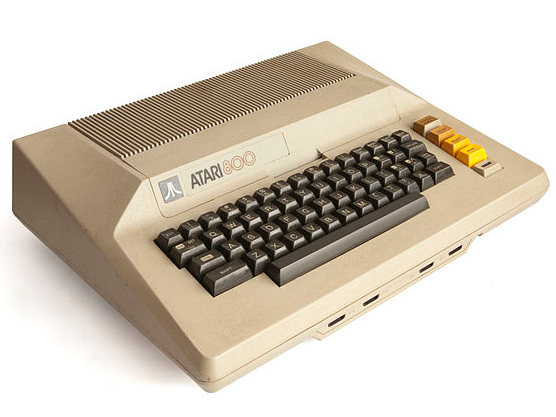
\includegraphics[width=\paperwidth,height=\paperheight]{atari-800}};
    % https://en.wikipedia.org/wiki/File:Atari_800.jpg
    % Wikimedia user Bilby
    % CC-BY-SA 3.0
    \node[above=5pt,black,fill=white,fill opacity=0.7,text opacity=0.8]
        at(current page.center)
        {8 bitů};
    \node[below=5pt,black,fill=white,fill opacity=0.7,text opacity=0.8]
        at(current page.center)
        {0-255};
    \attributionnode{© Wikimedia user Bilby, CC-BY-SA: \url{https://en.wikipedia.org/wiki/File:Atari_800.jpg}}
    \end{tikzpicture}
}

\frame[t]{
    \begin{tikzpicture}[remember picture,overlay]
    \path[use as bounding box] (0,0);
    % draw image
    \node[inner sep=0] at (current page.center)
        {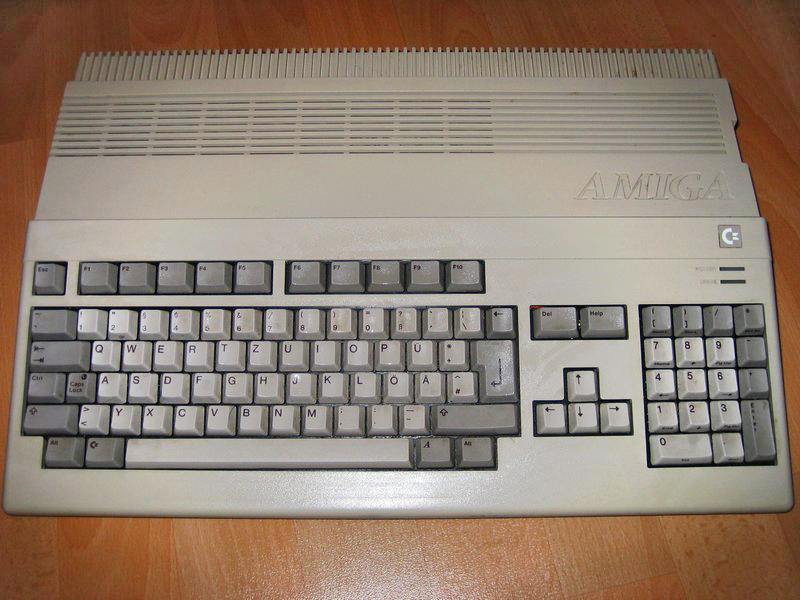
\includegraphics[width=\paperwidth,height=\paperheight]{amiga}};
    \node[above=5pt,black,fill=white,fill opacity=0.7,text opacity=0.8]
        at(current page.center)
        {16 bitů};
    \node[below=5pt,black,fill=white,fill opacity=0.7,text opacity=0.8]
        at(current page.center)
        {0-65\,535};
    % https://commons.wikimedia.org/wiki/File:Amiga_500_(1987).jpg
    % Dragan at the German language Wikipedia
    % CC-BY-SA 3.0
    \attributionnode{© Dragan at the German language Wikipedia, CC-BY-SA: \url{https://commons.wikimedia.org/wiki/File:Amiga_500_(1987).jpg}}
    \end{tikzpicture}
}

\frame[t]{
    \begin{tikzpicture}[remember picture,overlay]
    \path[use as bounding box] (0,0);
    % draw image
    \node[inner sep=0] at (current page.center)
        {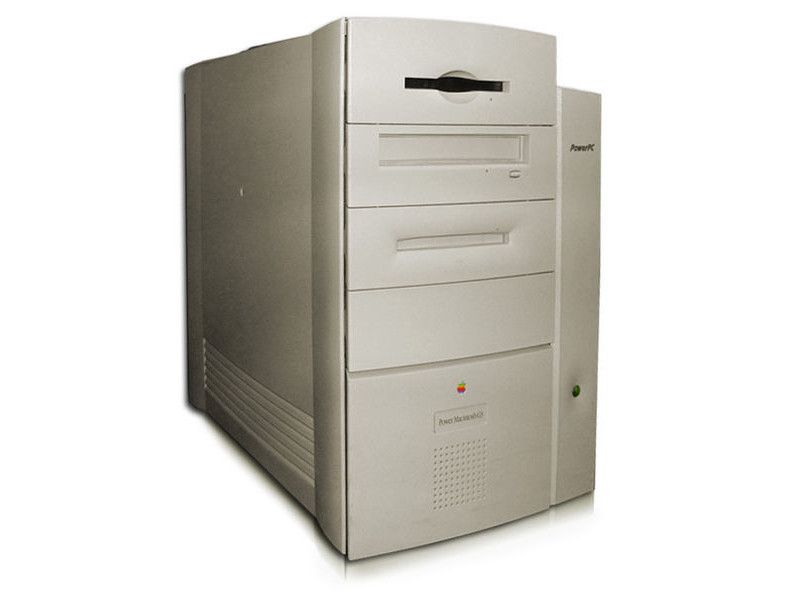
\includegraphics[width=\paperwidth,height=\paperheight]{beige-box}};
    \node[above=5pt,black,fill=white,fill opacity=0.7,text opacity=0.8]
        at(current page.center)
        {32 bitů};
    \node[below=5pt,black,fill=white,fill opacity=0.7,text opacity=0.8]
        at(current page.center)
        {0-4\,294\,967\,295};
    % https://en.wikipedia.org/wiki/File:Beige_Power_Macintosh_G3_Minitower.jpg
    % Public Domain
    \attributionnode{Public Domain image: \url{https://en.wikipedia.org/wiki/File:Beige_Power_Macintosh_G3_Minitower.jpg}}
    \end{tikzpicture}
}

\frame[t]{
    \begin{tikzpicture}[remember picture,overlay]
    \path[use as bounding box] (0,0);
    % draw image
    \node[inner sep=0] at (current page.center)
        {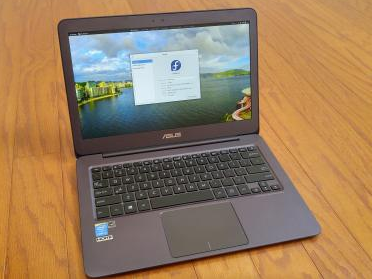
\includegraphics[width=\paperwidth,height=\paperheight]{laptop}};
    \node[above=5pt,black,fill=white,fill opacity=0.7,text opacity=0.8]
        at(current page.center)
        {64 bitů};
    \node[below=5pt,black,fill=white,fill opacity=0.7,text opacity=0.8]
        at(current page.center)
        {0-18\,446\,744\,073\,709\,551\,615};
    % https://opensource.com/life/15/8/beautiful-super-thin-laptop-makes-fedora-shine
    % Anderson Silva
    % CC BY-SA 4.0
    \attributionnode{© Anderson Silva, CC-BY-SA: \url{https://opensource.com/life/15/8/beautiful-super-thin-laptop-makes-fedora-shine}}
    \end{tikzpicture}
}

\frame[t]{

    \bigskip\bigskip
    \bigskip\bigskip
    \bigskip\bigskip

    8 bitů = 1 byte
}

\newcommand\dummy{
    \node[white,ellipse callout,draw=white, callout relative pointer={(0, -3mm)}]{\phantom{\flag{cz}}};
}
\newcommand\stor[1]{
    \node[black,ellipse callout,draw=black, callout relative pointer={(0, -3mm)}]{#1};
}
\newcommand\load[1]{
    \node[black,ellipse callout,draw=black, callout relative pointer={(0, 3mm)}]{#1};
}
\newcommand\dummyt{
    \node[white,ellipse callout,draw=white, callout relative pointer={(0, 3mm)}]{\phantom{\flag{cz}}};
}
\newcommand\dummyx{
    \node[white,ellipse callout,draw=white, callout relative pointer={(0, 3mm)}]{\phantom{J}};
}
\newcommand\bbdef{\useasboundingbox (0,0) -- (1mm, 1mm);}
\newcommand\flag[1]{\includegraphics[height=0.9em]{flags/#1}}
\newcommand\colr[1]{\textcolor{#1}\faCircle}

\begin{frame}[fragile]
    \tiny

    \leftskip-0.8in
    \begin{tikzpicture}
      \bbdef
      \matrix {
        & \dummy \\
        \node{0}; & \node{1}; & \node{2}; & \node{3}; & \node{4};  & \node{5}; \\
        \node[ta3aluminium,draw=black] {00000000}; &
        \node[ta3aluminium,draw=black] {00000000}; &
        \node[ta3aluminium,draw=black] {00000000}; &
        \node[ta3aluminium,draw=black] {00000000}; &
        \node[ta3aluminium,draw=black] {00000000}; &
        \node[ta3aluminium,draw=black] {00000000}; \\
      };
    \end{tikzpicture}
\end{frame}

\begin{frame}[fragile]
    \tiny

    \leftskip-0.8in
    \begin{tikzpicture}
      \bbdef
      \matrix {
        & \stor{29}; \\
        \node{0}; & \node{1}; & \node{2}; & \node{3}; & \node{4};  & \node{5}; \\
        \node[ta3aluminium,draw=black] {00000000}; &
        \node[draw=black] {00011101}; &
        \node[ta3aluminium,draw=black] {00000000}; &
        \node[ta3aluminium,draw=black] {00000000}; &
        \node[ta3aluminium,draw=black] {00000000}; &
        \node[ta3aluminium,draw=black] {00000000}; \\
        \dummyt; \\
        \dummyt; \\
        \dummyt; \\
        \dummyt; \\
      };
    \end{tikzpicture}
\end{frame}

\begin{frame}[fragile]
    \tiny

    \leftskip-0.8in
    \begin{tikzpicture}
      \bbdef
      \matrix {
        & \stor{29}; & \stor{'P'}; \\
        \node{0}; & \node{1}; & \node{2}; & \node{3}; & \node{4};  & \node{5}; \\
        \node[ta3aluminium,draw=black] {00000000}; &
        \node[draw=black] {00011101}; &
        \node[draw=black] {01010000}; &
        \node[ta3aluminium,draw=black] {00000000}; &
        \node[ta3aluminium,draw=black] {00000000}; &
        \node[ta3aluminium,draw=black] {00000000}; \\
        \dummyt; \\
        \dummyt; \\
        \dummyt; \\
        \dummyt; \\
      };
    \end{tikzpicture}
\end{frame}

\begin{frame}[fragile]
    \tiny

    \leftskip-0.8in
    \begin{tikzpicture}
      \bbdef
      \matrix {
        & \stor{29}; & \stor{'P'}; & \stor{
\includegraphics[height=0.9em]{flags/cz}}; \\
        \node{0}; & \node{1}; & \node{2}; & \node{3}; & \node{4};  & \node{5}; \\
        \node[ta3aluminium,draw=black] {00000000}; &
        \node[draw=black] {00011101}; &
        \node[draw=black] {01010000}; &
        \node[draw=black] {00101110}; &
        \node[ta3aluminium,draw=black] {00000000}; &
        \node[ta3aluminium,draw=black] {00000000}; \\
        \dummyt; \\
        \dummyt; \\
        \dummyt; \\
        \dummyt; \\
      };
    \end{tikzpicture}
\end{frame}

\begin{frame}[fragile]
    \tiny

    \leftskip-0.8in
    \begin{tikzpicture}
      \bbdef
      \matrix {
        & \stor{29}; & \stor{'P'}; & \stor{
\includegraphics[height=0.9em]{flags/cz}}; & 
        \stor{{\textcolor{yellow}\faCircle}};
        \\
        \node{0}; & \node{1}; & \node{2}; & \node{3}; & \node{4};  & \node{5}; \\
        \node[ta3aluminium,draw=black] {00000000}; &
        \node[draw=black] {00011101}; &
        \node[draw=black] {01010000}; &
        \node[draw=black] {00101110}; &
        \node[draw=black] {00111100}; &
        \node[ta3aluminium,draw=black] {00000000}; \\
        \dummyt; \\
        \dummyt; \\
        \dummyt; \\
        \dummyt; \\
      };
      \bbdef
    \end{tikzpicture}
\end{frame}

\begin{frame}[fragile]
    \tiny

    \leftskip-0.8in
    \begin{tikzpicture}
     \bbdef
     \matrix {
        & \stor{29}; & \stor{'P'}; & \stor{
\includegraphics[height=0.9em]{flags/cz}}; & 
        \stor{{\textcolor{yellow}\faCircle}};
        \\
        \node{0}; & \node{1}; & \node{2}; & \node{3}; & \node{4};  & \node{5}; \\
        \node[ta3aluminium,draw=black] {00000000}; &
        \node[draw=black] {00011101}; &
        \node[draw=black] {01010000}; &
        \node[draw=black] {00101110}; &
        \node[draw=black] {00111100}; &
        \node[ta3aluminium,draw=black] {00000000}; \\
        \dummyt; & \load{29}; & \load{80}; & \load{46}; & \load{60}; \\
        \dummyt; \\
        \dummyt; \\
        \dummyt; \\
      };
    \end{tikzpicture}
\end{frame}

\begin{frame}[fragile]
    {}\tiny

    \leftskip-0.8in
    \begin{tikzpicture}
      \bbdef
      \matrix {
        & \stor{29}; & \stor{'P'}; & \stor{
\includegraphics[height=0.9em]{flags/cz}}; & 
        \stor{{\textcolor{yellow}\faCircle}};
        \\
        \node{0}; & \node{1}; & \node{2}; & \node{3}; & \node{4};  & \node{5}; \\
        \node[ta3aluminium,draw=black] {00000000}; &
        \node[draw=black] {00011101}; &
        \node[draw=black] {01010000}; &
        \node[draw=black] {00101110}; &
        \node[draw=black] {00111100}; &
        \node[ta3aluminium,draw=black] {00000000}; \\
        \dummyt; & \load{29}; & \load{80}; & \load{46}; & \load{60}; \\
        \dummyt; & \load{'\faArrowsH'}; & \load{'P'}; & \load{'.'}; & \load{'<'}; \\
        \dummyt; \\
        \dummyt; \\
      };
    \end{tikzpicture}
\end{frame}

\begin{frame}[fragile]
    {}\tiny

    \leftskip-0.8in
    \begin{tikzpicture}
      \bbdef
      \matrix {
        & \stor{29}; & \stor{'P'}; & \stor{\flag{cz}}; & 
        \stor{{\textcolor{yellow}\faCircle}};
        \\
        \node{0}; & \node{1}; & \node{2}; & \node{3}; & \node{4};  & \node{5}; \\
        \node[ta3aluminium,draw=black] {00000000}; &
        \node[draw=black] {00011101}; &
        \node[draw=black] {01010000}; &
        \node[draw=black] {00101110}; &
        \node[draw=black] {00111100}; &
        \node[ta3aluminium,draw=black] {00000000}; \\
        \dummyt; & \load{29}; & \load{80}; & \load{46}; & \load{60}; \\
        \dummyt; & \load{'\faArrowsH'}; & \load{'P'}; & \load{'.'}; & \load{'<'}; \\
        \dummyt; & \load{\flag{cv}}; & \load{\flag{ir}}; & \load{\flag{cz}}; & \load{\flag{fr}}; \\
        \dummyt; \\
      };
    \end{tikzpicture}
\end{frame}

\begin{frame}[fragile]
    {}\tiny

    \leftskip-0.8in
    \begin{tikzpicture}
      \bbdef
      \matrix {
        & \stor{29}; & \stor{'P'}; & \stor{\flag{cz}}; & 
        \stor{\colr{yellow}};
        \\
        \node{0}; & \node{1}; & \node{2}; & \node{3}; & \node{4};  & \node{5}; \\
        \node[ta3aluminium,draw=black] {00000000}; &
        \node[draw=black] {00011101}; &
        \node[draw=black] {01010000}; &
        \node[draw=black] {00101110}; &
        \node[draw=black] {00111100}; &
        \node[ta3aluminium,draw=black] {00000000}; \\
        \dummyt; & \load{29}; & \load{80}; & \load{46}; & \load{60}; \\
        \dummyt; & \load{'\faArrowsH'}; & \load{'P'}; & \load{'.'}; & \load{'<'}; \\
        \dummyt; & \load{\flag{cv}}; & \load{\flag{ir}}; & \load{\flag{cz}}; & \load{\flag{fr}}; \\
        \dummyt; & \load{\colr{green!50!white}}; & \load{\colr{red!50!black}}; & \load{\colr{yellow!50!white}}; & \load{\colr{yellow}}; \\
      };
    \end{tikzpicture}
\end{frame}

\begin{frame}[fragile]
    {}\tiny

    \leftskip-0.8in
    \begin{tikzpicture}
      \bbdef
      \matrix {
        \node{0}; & \node{1}; & \node{2}; & \node{3}; & \node{4};  & \node{5}; & \node{6}; \\
        \node[ta3aluminium,draw=black] {00000000}; &
        \node[ta3aluminium,draw=black] {00000000}; &
        \node[draw=black] {01000001}; &
        \node[draw=black] {01101000}; &
        \node[draw=black] {00111100}; &
        \node[draw=black] {01101111}; &
        \node[draw=black] {00000000}; \\
         && \load{65}; & \load{104}; & \load{111}; & \load{106}; & \load{0}; \\
         && \load{'A'}; & \load{'h'}; & \load{'o'}; & \load{'j'}; & \load{\faRemove}; \\
      };
    \end{tikzpicture}
\end{frame}

\begin{frame}[fragile]
    {}\tiny

    \leftskip-0.8in
    \begin{tikzpicture}
      \bbdef
      \matrix {
        \node{0}; & \node{1}; & \node{2}; & \node{3}; & \node{4};  & \node{5}; & \node{6}; \\
        \node[ta3aluminium,draw=black] {00000000}; &
        \node[draw=black] {00000004}; &
        \node[draw=black] {01000001}; &
        \node[draw=black] {01101000}; &
        \node[draw=black] {00111100}; &
        \node[draw=black] {01101111}; &
        \node[draw=black] {00000000}; \\
         & \load{4}; & \load{65}; & \load{104}; & \load{111}; & \load{106}; & \load{0}; \\
         & \node{délka}; & \load{'A'}; & \load{'h'}; & \load{'o'}; & \load{'j'}; & \load{\faRemove}; \\
      };
    \end{tikzpicture}
\end{frame}

\begin{frame}[fragile]
    {}\tiny

    \leftskip-0.8in
    \begin{tikzpicture}
      \bbdef
      \matrix {
        \node{0}; & \node{1}; & \node{2}; & \node{3}; & \node{4};  & \node{5}; & \node{6}; \\
        \node[draw=black] {10010010}; &
        \node[draw=black] {00000004}; &
        \node[draw=black] {01000001}; &
        \node[draw=black] {01101000}; &
        \node[draw=black] {00111100}; &
        \node[draw=black] {01101111}; &
        \node[draw=black] {00000000}; \\
        \load{146} & \load{4}; & \load{65}; & \load{104}; & \load{111}; & \load{106}; & \load{0}; \\
        \load{\texttt{str}} & \node{délka}; & \load{'A'}; & \load{'h'}; & \load{'o'}; & \load{'j'}; & \load{\faRemove}; \\
      };
    \end{tikzpicture}
\end{frame}

\begin{frame}[fragile]
    {}\tiny

    \leftskip-0.8in
    \begin{tikzpicture}
      \useasboundingbox (0,0) -- (1mm, -5cm);

      \matrix {
        \node{0}; & \node{1}; & \node{2}; & \node{3}; & \node{4};  & \node{5}; & \node{6}; \\
        \node[draw=black] (strstart) {10010010}; &
        \node[draw=black] {00000004}; &
        \node[draw=black] {01000001}; &
        \node[draw=black] {01101000}; &
        \node[draw=black] {00111100}; &
        \node[draw=black] {01101111}; &
        \node[draw=black] {00000000}; \\
        \load{146} & \load{4}; & \load{65}; & \load{104}; & \load{111}; & \load{106}; & \load{0}; \\
        \load{\texttt{str}} & \node{délka}; & \load{'A'}; & \load{'h'}; & \load{'o'}; & \load{'j'}; & \load{\faRemove}; \\
      };

      \matrix at (0, -5cm) {
        \node{146}; & \node{147}; & \node{148}; & \node{149}; & \node{150};  & \node{151}; & \node{152}; \\
        \node[draw=black] (typestart) {10011010}; &
        \node[ta3aluminium,draw=black] {11101100}; &
        \node[ta3aluminium,draw=black] {11001111}; &
        \node[ta3aluminium,draw=black] {11001100}; &
        \node[ta3aluminium,draw=black] {11011010}; &
        \node[ta3aluminium,draw=black] {11100011}; &
        \node[ta3aluminium,draw=black] {10101101}; \\
        % \load{154} & \load{236}; & \load{207}; & \load{204}; & \load{218}; & \load{227}; & \load{173}; \\
        \load{\texttt{type}} & \node {...}; & \node {...}; & \node {...}; & \node {...}; \\
      };
      \draw[thick] (strstart.south west) edge[bend right=15,->] (typestart.north west);
    \end{tikzpicture}
\end{frame}

\newcommand\ld[1]{
    \node[draw opacity=0,minimum size=1mm] {#1};
}
\begin{frame}[fragile]
    {}\tiny

    \leftskip-0.8in
    
\begin{tikzpicture}[every node/.style={minimum size=1cm,draw,anchor=base,text height=.8em,text depth=.2em}]

      \matrix {
        \ld{A} & \node {}; & \node {}; & \node {}; & \node {}; & \node {}; & \node {}; & \node {}; & \node {}; \\
        \ld{B} & \node {}; & \node {}; & \node {}; & \node {}; & \node {}; & \node {}; & \node {}; & \node {}; \\
        \ld{C} & \node {}; & \node {}; & \node {}; & \node {}; & \node {}; & \node {}; & \node {}; & \node {}; \\
        \ld{D} & \node {}; & \node {}; & \node {}; & \node {}; & \node {}; & \node {}; & \node {}; & \node {}; \\
        \ld{E} & \node {}; & \node {}; & \node {}; & \node {}; & \node {}; & \node {}; & \node {}; & \node {}; \\
        \ld{F} & \node {}; & \node {}; & \node {}; & \node {}; & \node {}; & \node {}; & \node {}; & \node {}; \\
        \ld{G} & \node {}; & \node {}; & \node {}; & \node {}; & \node {}; & \node {}; & \node {}; & \node {}; \\
        \ld{H} & \node {}; & \node {}; & \node {}; & \node {}; & \node {}; & \node {}; & \node {}; & \node {}; \\
&\ld{0}&\ld{1}&\ld{2}&\ld{3}&\ld{4}&\ld{5}&\ld{6}&\ld{7}\\
      };
    \end{tikzpicture}
\end{frame}

% % % 
% % % \begin{frame}[fragile]
% % %     {}\tiny
% % % 
% % %     \leftskip-0.8in
% % %     \begin{tikzpicture}[every node/.style={minimum size=1cm,draw,anchor=base,text height=.8em,text depth=.2em}]
% % % 
% % %       \matrix {
% % %         \ld{A} & \node {\textit{G0}}; & \node {4}; & \node {'A'}; & \node {'h'}; & \node {'o'}; & \node {'j'}; & \node {\faRemove}; & \node {}; \\
% % %         \ld{B} & \node {}; & \node {}; & \node {}; & \node {}; & \node {}; & \node {}; & \node {}; & \node {}; \\
% % %         \ld{C} & \node {}; & \node {}; & \node {}; & \node {}; & \node {}; & \node {}; & \node {}; & \node {}; \\
% % %         \ld{D} & \node {}; & \node {}; & \node {}; & \node {}; & \node {}; & \node {}; & \node {}; & \node {}; \\
% % %         \ld{E} & \node {}; & \node {}; & \node {}; & \node {}; & \node {}; & \node {}; & \node {}; & \node {}; \\
% % %         \ld{F} & \node {}; & \node {}; & \node {}; & \node {}; & \node {}; & \node {}; & \node {}; & \node {}; \\
% % %         \ld{G} & \node {\textit{H0}}; & \node {str}; & \node {...}; & \node {...}; & \node {}; & \node {}; & \node {}; & \node {}; \\
% % %         \ld{H} & \node {\textit{H0}}; & \node {type}; & \node {...}; & \node {...}; & \node {}; & \node {}; & \node {}; & \node {}; \\
% % %         &\ld{0}&\ld{1}&\ld{2}&\ld{3}&\ld{4}&\ld{5}&\ld{6}&\ld{7}\\
% % %       };
% % %     \end{tikzpicture}
% % % \end{frame}

\begin{frame}[fragile]
    {}\tiny

    \leftskip-0.8in
    \begin{tikzpicture}[every node/.style={minimum size=1cm,draw,anchor=base,text height=.8em,text depth=.2em}]

      \matrix {
        \ld{A} & \node {str}; & \node {4}; & \node {'A'}; & \node {'h'}; & \node {'o'}; & \node {'j'}; & \node {\faRemove}; & \node {}; \\
        \ld{B} & \node {}; & \node {}; & \node {}; & \node {}; & \node {}; & \node {}; & \node {}; & \node {}; \\
        \ld{C} & \node {}; & \node {}; & \node {}; & \node {}; & \node {}; & \node {}; & \node {}; & \node {}; \\
        \ld{D} & \node {}; & \node {}; & \node {}; & \node {}; & \node {}; & \node {}; & \node {}; & \node {}; \\
        \ld{E} & \node {}; & \node {}; & \node {}; & \node {}; & \node {}; & \node {}; & \node {}; & \node {}; \\
        \ld{F} & \node {}; & \node {}; & \node {}; & \node {}; & \node {}; & \node {}; & \node {}; & \node {}; \\
        \ld{G} & \node {}; & \node {}; & \node {}; & \node {}; & \node {}; & \node {}; & \node {}; & \node {}; \\
        \ld{H} & \node {}; & \node {}; & \node {}; & \node {}; & \node {}; & \node {}; & \node {}; & \node {}; \\
        &\ld{0}&\ld{1}&\ld{2}&\ld{3}&\ld{4}&\ld{5}&\ld{6}&\ld{7}\\
      };
      \node[align=left,draw opacity=0,below right,minimum size=3cm] at (4cm, 7cm)
        {A0: "ahoj"};
    \end{tikzpicture}
\end{frame}

\begin{frame}[fragile]
    {}\tiny

    \leftskip-0.8in
    \begin{tikzpicture}[every node/.style={minimum size=1cm,draw,anchor=base,text height=.8em,text depth=.2em}]

      \matrix {
        \ld{A} & \node {str}; & \node {4}; & \node {'A'}; & \node {'h'}; & \node {'o'}; & \node {'j'}; & \node {\faRemove}; & \node {}; \\
        \ld{B} & \node {int}; & \node {1}; & \node {0}; & \node {}; & \node {int}; & \node {1}; & \node {1}; & \node {}; \\
        \ld{C} & \node {}; & \node {}; & \node {}; & \node {}; & \node {}; & \node {}; & \node {}; & \node {}; \\
        \ld{D} & \node {}; & \node {}; & \node {}; & \node {}; & \node {}; & \node {}; & \node {}; & \node {}; \\
        \ld{E} & \node {}; & \node {}; & \node {}; & \node {}; & \node {}; & \node {}; & \node {}; & \node {}; \\
        \ld{F} & \node {}; & \node {}; & \node {}; & \node {}; & \node {}; & \node {}; & \node {}; & \node {}; \\
        \ld{G} & \node {}; & \node {}; & \node {}; & \node {}; & \node {}; & \node {}; & \node {}; & \node {}; \\
        \ld{H} & \node {}; & \node {}; & \node {}; & \node {}; & \node {}; & \node {}; & \node {}; & \node {}; \\
        &\ld{0}&\ld{1}&\ld{2}&\ld{3}&\ld{4}&\ld{5}&\ld{6}&\ld{7}\\
      };
      \node[align=left,draw opacity=0,below right,minimum size=3cm] at (4cm, 7cm)
        {A0: "ahoj" \\ B0: 0 \\ B4: 1};
    \end{tikzpicture}
\end{frame}

\begin{frame}[fragile]
    {}\tiny

    \leftskip-0.8in
    \begin{tikzpicture}[every node/.style={minimum size=1cm,draw,anchor=base,text height=.8em,text depth=.2em}]

      \matrix {
        \ld{A} & \node {str}; & \node {4}; & \node {'A'}; & \node {'h'}; & \node {'o'}; & \node {'j'}; & \node {\faRemove}; & \node {}; \\
        \ld{B} & \node {int}; & \node {1}; & \node {0}; & \node {}; & \node {int}; & \node {1}; & \node {1}; & \node {}; \\
        \ld{C} & \node {tupl}; & \node {2}; & \node {\textit{B0}}; & \node {\textit{B4}}; & \node {}; & \node {}; & \node {}; & \node {}; \\
        \ld{D} & \node {}; & \node {}; & \node {}; & \node {}; & \node {}; & \node {}; & \node {}; & \node {}; \\
        \ld{E} & \node {}; & \node {}; & \node {}; & \node {}; & \node {}; & \node {}; & \node {}; & \node {}; \\
        \ld{F} & \node {}; & \node {}; & \node {}; & \node {}; & \node {}; & \node {}; & \node {}; & \node {}; \\
        \ld{G} & \node {}; & \node {}; & \node {}; & \node {}; & \node {}; & \node {}; & \node {}; & \node {}; \\
        \ld{H} & \node {}; & \node {}; & \node {}; & \node {}; & \node {}; & \node {}; & \node {}; & \node {}; \\
        &\ld{0}&\ld{1}&\ld{2}&\ld{3}&\ld{4}&\ld{5}&\ld{6}&\ld{7}\\
      };
      \node[align=left,draw opacity=0,below right,minimum size=3cm] at (4cm, 7cm)
        {A0: "ahoj" \\ B0: 0 \\ B4: 1 \\ C0: (0, 1)};
    \end{tikzpicture}
\end{frame}

\begin{frame}[fragile]
    {}\tiny

    \leftskip-0.8in
    \begin{tikzpicture}[every node/.style={minimum size=1cm,draw,anchor=base,text height=.8em,text depth=.2em}]

      \matrix {
        \ld{A} & \node {str}; & \node {4}; & \node {'A'}; & \node {'h'}; & \node {'o'}; & \node {'j'}; & \node {\faRemove}; & \node {}; \\
        \ld{B} & \node {int}; & \node {1}; & \node {0}; & \node {}; & \node {int}; & \node {1}; & \node {1}; & \node {}; \\
        \ld{C} & \node {tupl}; & \node {2}; & \node {\textit{B0}}; & \node {\textit{B4}}; & \node {}; & \node {int}; & \node {1}; & \node {2}; \\
        \ld{D} & \node {}; & \node {}; & \node {}; & \node {}; & \node {}; & \node {}; & \node {}; & \node {}; \\
        \ld{E} & \node {}; & \node {}; & \node {}; & \node {}; & \node {}; & \node {}; & \node {}; & \node {}; \\
        \ld{F} & \node {}; & \node {}; & \node {}; & \node {}; & \node {}; & \node {}; & \node {}; & \node {}; \\
        \ld{G} & \node {}; & \node {}; & \node {}; & \node {}; & \node {}; & \node {}; & \node {}; & \node {}; \\
        \ld{H} & \node {}; & \node {}; & \node {}; & \node {}; & \node {}; & \node {}; & \node {}; & \node {}; \\
        &\ld{0}&\ld{1}&\ld{2}&\ld{3}&\ld{4}&\ld{5}&\ld{6}&\ld{7}\\
      };
      \node[align=left,draw opacity=0,below right,minimum size=3cm] at (4cm, 7cm)
        {A0: "ahoj" \\ B0: 0 \\ B4: 1 \\ C0: (0, 1) \\ C5: 2};
    \end{tikzpicture}
\end{frame}

\begin{frame}[fragile]
    {}\tiny

    \leftskip-0.8in
    \begin{tikzpicture}[every node/.style={minimum size=1cm,draw,anchor=base,text height=.8em,text depth=.2em}]

      \matrix {
        \ld{A} & \node {str}; & \node {4}; & \node {'A'}; & \node {'h'}; & \node {'o'}; & \node {'j'}; & \node {\faRemove}; & \node {}; \\
        \ld{B} & \node {int}; & \node {1}; & \node {0}; & \node {}; & \node {int}; & \node {1}; & \node {1}; & \node {}; \\
        \ld{C} & \node {tupl}; & \node {2}; & \node {\textit{B0}}; & \node {\textit{B4}}; & \node {}; & \node {int}; & \node {1}; & \node {2}; \\
        \ld{D} & \node {lst}; & \node {3}; & \node {\textit{E4}}; & \node {}; & \node {}; & \node {}; & \node {}; & \node {}; \\
        \ld{E} & \node {}; & \node {}; & \node {}; & \node {}; & \node {\textit{B0}}; & \node {\textit{B4}}; & \node {\textit{C5}}; & \node {\faRemove}; \\
        \ld{F} & \node {}; & \node {}; & \node {}; & \node {}; & \node {}; & \node {}; & \node {}; & \node {}; \\
        \ld{G} & \node {}; & \node {}; & \node {}; & \node {}; & \node {}; & \node {}; & \node {}; & \node {}; \\
        \ld{H} & \node {}; & \node {}; & \node {}; & \node {}; & \node {}; & \node {}; & \node {}; & \node {}; \\
        &\ld{0}&\ld{1}&\ld{2}&\ld{3}&\ld{4}&\ld{5}&\ld{6}&\ld{7}\\
      };
      \node[align=left,draw opacity=0,below right,minimum size=3cm] at (4cm, 7cm)
        {A0: "ahoj" \\ B0: 0 \\ B4: 1 \\ C0: (0, 1) \\ C5: 2 \\ D0: [0, 1, 2]};
    \end{tikzpicture}
\end{frame}

\begin{frame}[fragile]
    {}\tiny

    \leftskip-0.8in
    \begin{tikzpicture}[every node/.style={minimum size=1cm,draw,anchor=base,text height=.8em,text depth=.2em}]

      \matrix {
        \ld{A} & \node {str}; & \node {4}; & \node {'A'}; & \node {'h'}; & \node {'o'}; & \node {'j'}; & \node {\faRemove}; & \node {}; \\
        \ld{B} & \node {int}; & \node {1}; & \node {0}; & \node {}; & \node {int}; & \node {1}; & \node {1}; & \node {}; \\
        \ld{C} & \node {tupl}; & \node {2}; & \node {\textit{B0}}; & \node {\textit{B4}}; & \node {}; & \node {int}; & \node {1}; & \node {2}; \\
        \ld{D} & \node {lst}; & \node {4}; & \node {\textit{F1}}; & \node {}; & \node {}; & \node {}; & \node {}; & \node {}; \\
        \ld{E} & \node {}; & \node {}; & \node {}; & \node {}; & \node {{\textcolor{ta3aluminium}{\textit B0}}}; & \node {{\textcolor{ta3aluminium}{\textit B4}}}; & \node {{\textcolor{ta3aluminium}{\textit C5}}}; & \node {{\textcolor{ta3aluminium}{\faRemove}}}; \\
        \ld{F} & \node {}; & \node {\textit{B0}}; & \node {\textit{B4}}; & \node {\textit{C5}}; & \node {\textit{B0}}; & \node {\faRemove}; & \node {}; & \node {}; \\
        \ld{G} & \node {}; & \node {}; & \node {}; & \node {}; & \node {}; & \node {}; & \node {}; & \node {}; \\
        \ld{H} & \node {}; & \node {}; & \node {}; & \node {}; & \node {}; & \node {}; & \node {}; & \node {}; \\
        &\ld{0}&\ld{1}&\ld{2}&\ld{3}&\ld{4}&\ld{5}&\ld{6}&\ld{7}\\
      };
      \node[align=left,draw opacity=0,below right,minimum size=3cm] at (4cm, 7cm)
        {A0: "ahoj" \\ B0: 0 \\ B4: 1 \\ C0: (0, 1) \\ C5: 2 \\ D0: [0,1,2,0]};
    \end{tikzpicture}
\end{frame}

\begin{frame}[fragile]
    {}\tiny

    \leftskip-0.8in
    
\begin{tikzpicture}[every node/.style={minimum size=1cm,draw,anchor=base,text height=.8em,text depth=.2em}]

      \matrix {
        \ld{A} & \node {}; & \node {}; & \node {}; & \node {}; & \node {}; & \node {}; & \node {}; & \node {}; \\
        \ld{B} & \node {}; & \node {}; & \node {}; & \node {}; & \node {}; & \node {}; & \node {}; & \node {}; \\
        \ld{C} & \node {}; & \node {}; & \node {}; & \node {}; & \node {}; & \node {}; & \node {}; & \node {}; \\
        \ld{D} & \node {}; & \node {}; & \node {}; & \node {}; & \node {}; & \node {}; & \node {}; & \node {}; \\
        \ld{E} & \node {}; & \node {}; & \node {}; & \node {}; & \node {}; & \node {}; & \node {}; & \node {}; \\
        \ld{F} & \node {}; & \node {}; & \node {}; & \node {}; & \node {}; & \node {}; & \node {}; & \node {}; \\
        \ld{G} & \node {}; & \node {}; & \node {}; & \node {}; & \node {}; & \node {}; & \node {}; & \node {}; \\
        \ld{H} & \node {}; & \node {}; & \node {}; & \node {}; & \node {}; & \node {}; & \node {}; & \node {}; \\
        &\ld{0}&\ld{1}&\ld{2}&\ld{3}&\ld{4}&\ld{5}&\ld{6}&\ld{7}\\
      };
    \end{tikzpicture}
\end{frame}

\begin{frame}[fragile]
    {}\tiny

    \leftskip-0.8in
    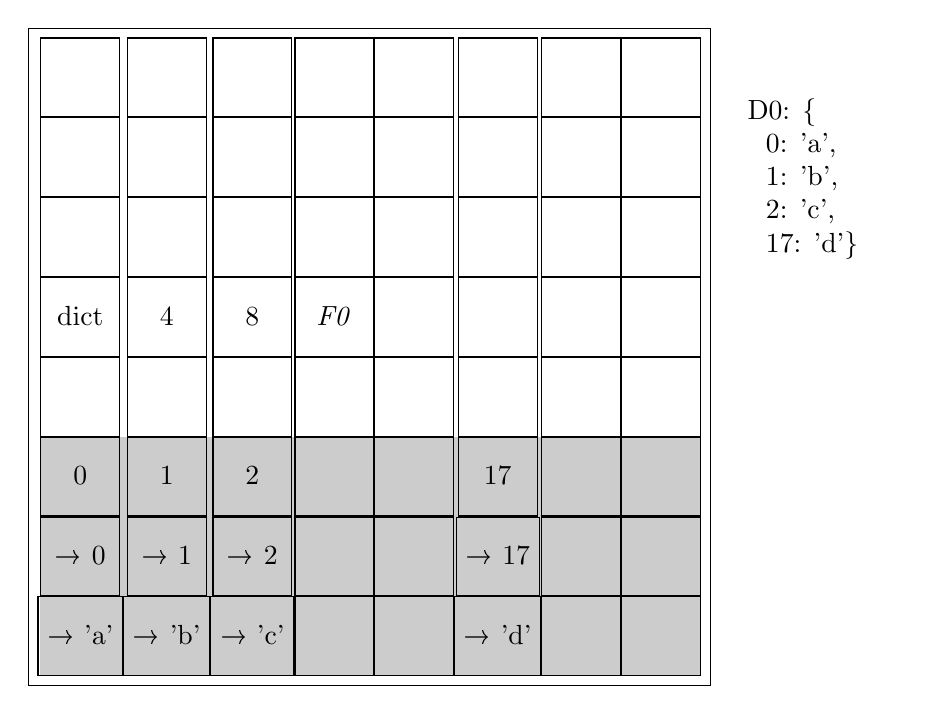
\begin{tikzpicture}[every node/.style={minimum size=1cm,draw,anchor=base,text height=.8em,text depth=.2em}]

      \matrix {
        \ld{A} & \node {}; & \node {}; & \node {}; & \node {}; & \node {}; & \node {}; & \node {}; & \node {}; \\
        \ld{B} & \node {}; & \node {}; & \node {}; & \node {}; & \node {}; & \node {}; & \node {}; & \node {}; \\
        \ld{C} & \node {}; & \node {}; & \node {}; & \node {}; & \node {}; & \node {}; & \node {}; & \node {}; \\
        \ld{D} & \node {dict}; & \node {4}; & \node {8}; & \node {\textit{F0}}; & \node {}; & \node {}; & \node {}; & \node {}; \\
        \ld{E} & \node {}; & \node {}; & \node {}; & \node {}; & \node {}; & \node {}; & \node {}; & \node {}; \\
        \ld{F} & \node (s) {0}; & \node {1}; & \node {2}; & \node {}; & \node {}; & \node {17}; & \node {}; & \node {}; \\
        \ld{G} & \node {→ 0}; & \node {→ 1}; & \node {→ 2}; & \node {}; & \node {}; & \node {→ 17}; & \node {}; & \node {}; \\
        \ld{H} & \node {→ 'a'}; & \node {→ 'b'}; & \node {→ 'c'}; & \node {}; & \node {}; & \node {→ 'd'}; & \node {}; & \node (e) {}; \\
        &\ld{0}&\ld{1}&\ld{2}&\ld{3}&\ld{4}&\ld{5}&\ld{6}&\ld{7}\\
      };
      \node[align=left,draw opacity=0,below right,minimum size=3cm] at (4cm, 7cm)
        {D0: \{ \\~~0: 'a', \\ ~~1: 'b',\\ ~~2: 'c', \\ ~~17: 'd'\}};
      \path[draw opacity=0,fill opacity=0.2,fill=black] (s.north west) rectangle (e.south east);
    \end{tikzpicture}
\end{frame}

\frame{

    \bigskip\bigskip
    \bigskip\bigskip
    \bigskip\bigskip

    {\huge ?}

    \bigskip\bigskip
    \bigskip

    {\tiny
    Petr Viktorin\\[10pt]%
    \href{http://encukou.cz}{@\rd{1}{encukou}.cz}\\%
    \href{mailto:encukou@gmail.com}{\rd{1}{encukou}@gmail.com}\\%
    \href{http://twitter.com/encukou}{@\rd{1}{encukou}}\\%
    \href{http://github.com/encukou}{github.com/\rd{1}{encukou}}\\%
    \sk
    \tx{1}{Licence: \\ Creative Commons Attribution-ShareAlike 4.0 \url{http://creativecommons.org/licenses/by-sa/4.0/}}\\
    }

}

% \frame{
%     \small
%     \rd{1}{Zdroje} \& odkazy\\[0.25cm]
%     \bigskip\bigskip
%     \tiny
%     %\tx{1}{\url{}}\\[0.25cm]
%     %\tx{1}{\url{}}\\[0.25cm]
%     %\bigskip
%     %\tx{1}{\url{}}\\[0.25cm]
%     %\tx{1}{\url{}}\\[0.25cm]
%     %\tx{1}{\url{}}\\[0.25cm]
% }

\end{center}
\end{document}

